\documentclass[conference]{IEEEtran}
\IEEEoverridecommandlockouts
% The preceding line is only needed to identify funding in the first footnote. If that is unneeded, please comment it out.
\usepackage{cite}
\usepackage{amsmath,amssymb,amsfonts}
\usepackage{algorithmic}
\usepackage{graphicx}
\usepackage[labelformat=parens, labelsep=space]{subcaption}
% \renewcommand\thesubfigure{(\alph{subfigure})}
\usepackage{textcomp}
\usepackage[table, xcdraw]{xcolor} % The cell in the table can be highlighted
\usepackage{booktabs} % Use book tab style for all tables
\usepackage{lettrine} % Capticalize the first letter in the paper

% Fix error when there is no bib item.
\def\BibTeX{{\rm B\kern-.05em{\sc i\kern-.025em b}\kern-.08em
    T\kern-.1667em\lower.7ex\hbox{E}\kern-.125emX}}

\makeatletter
\def\endthebibliography{%
  \def\@noitemerr{\@latex@warning{Empty `thebibliography' environment}}%
  \endlist
}

% Add a horizontal line for footnotes(thanks)
\def\footnoterule{\relax%
  \kern-5pt
  \hbox to \columnwidth{\hfill\vrule width 0.6\columnwidth height 0.4pt\hfill}
  \kern4.6pt}
\makeatother

\graphicspath{{figures/}}
\newtheorem{definition}{Definition}
\begin{document}
\title{Multi-modal Multi-objective Optimization: Problem Analysis and Case Studies
}
\author{\IEEEauthorblockN{Yiming Peng, Hisao Ishibuchi, Ke Shang}
\thanks{Y. Peng, H. Ishibuchi and K. Shang are with Shenzhen Key Laboratory of Computational Intelligence, University Key Laboratory of Evolving Intelligent Systems of Guangdong Province, Department of Computer Science and Engineering, Southern University of Science and Technology, Shenzhen 518055, China. e-mail: (rt.11510035@mail.sustech.edu.cn, hisao@sustech.edu.cn, kshang@foxmail.com). (Corresponding author: Hisao Ishibuchi)}
}

\maketitle

\begin{abstract}
In many real-world applications, multi-objective optimization problems can contain more than one Pareto sets. The optimization goal of multi-modal multi-objective optimization is to find all Pareto sets in the decision space. As a relatively new research area, the difficulties to solve multi-modal multi-objective optimization problem has not been carefully analyzed in literature. In this paper, we point out that traditional environmental selection, mutation and crossover mechanisms may cause problems when solving multi-modal multi-objective optimization problems. Furthermore, we creatively introduce the concept of genetic drift to explain the reduction of diversity in the decision space during the evolution process. In addiction, this paper also provides comparative studies of state-of-the-art algorithms using a series of computational experiments.
\end{abstract}

\begin{IEEEkeywords}
Multi-modal multi-objective optimization, Genetic Drift, Evolutionary algorithms
\end{IEEEkeywords}

\section{Introduction}
\lettrine[lines=2]{M}{any} real-world optimization problems require to optimize more than one objective functions which are usually conflict with each other. In most circumstances, the fitness improvement in one objective function will cause fitness deterioration in other objectives. We generally denote this kind of problems as Multi-objective Optimization Problems(MOPs). Multi-objective Evolutionary Algorithms(MOEAs) are designed for solving MOPs. Usually, MOEAs only consider the diversity of solution set in the objective space. Diversity in the decision space does not gain much attention. However, sometimes the diversity in the decision space is also very important, especially for multi-modal multi-objective optimization problems(MMOPs). MMOP is a special kind of MOPs which has more than one Pareto optimal solution sets(PS) corresponding to the same PF. There are many MMOPs in real-world applications such as multi-objective knapsack problems \cite{Jaszkiewicz2002}, game map generation problems \cite{Togelius} etc. An MMOP requires the optimizer to obtain a solution set that covers as more Pareto sets as possible. In many engineering problems, some solutions are hard to implement due to physical limitations. In this case, obtaining multiple Pareto sets can help the decision maker to select alternative solutions with equivalent quality in the objective space. In addition, the knowledge about multiple Pareto optimal solution sets may be helpful to better understand the structure of the optimization problem\cite{Deb2001}. For convenience, evolutionary algorithms designed for solving MMOPs are named as Multi-modal Multi-objective Evolutionary Algorithms or MMEAs for short.

As pointed out in many literature\cite{Tanabe2019} \cite{Liang2016}, MOEAs is not well-performed on MMOPs because they can only obtain a part of Pareto optimal solutions in most circumstances. In this paper, we further confirm this proposition with a series of computational experiments. In addition, we try to do some analysis and explanations on why MOEAs perform poor on MMOPs. We illustrate that in order to find solutions in all Pareto sets, an explicit mechanism to maintain the solution diversity in the decision space is necessary. This means that MMEAs should be able to preserve the diversity of the solutions in both decision and objective space. Since 2005, MMEAs has begun to draw attention from researchers in the MOEA community. Some new algorithms are specially designed for MMOPs and some of them are modified from existing MOEAs. In this paper, several popular MMEAs are tested and their performance on the test problems with different dimensional decision spaces is examined. We also examine the effectiveness of MMEAs on solving MMOPs compared with classical MOEAs.

The structure of this paper is organized as follows. In section \ref{Multi-modal Multi-objective Optimization}, we give the formal definition of MMOPs, and mainstream diversity maintenance techniques in the literature and their characteristics are reviewed. Section \ref{Difficulties Analysis} is devoted to analyze the difficulties of solving MMOPs. Then a series of computational experiments are conducted in section \ref{Experimental Studies}. Finally, we conclude this paper in section \ref{Conclusion}.
\section{Multi-modal Multi-objective Optimization}
\label{Multi-modal Multi-objective Optimization}
\subsection{Formal Definition}
The formal definition of MMOPs can be described as follows\cite{Tanabe2019}:
\begin{definition}
MMOP is a kind of MOP that aims to find all solutions that are equivalent to Pareto optimal solutions. 
\end{definition}
\begin{definition}
Solutions $\boldsymbol{x_1}$ and  $\boldsymbol{x_2}$ are equivalent  iff $||f(\boldsymbol{x_1}) - f(\boldsymbol{x_2})|| \leq \delta$ .
\end{definition}
Where $\delta$ is a positive number that represents the tolerance of similarity of solutions given by the decision maker. If $\delta = 0$, the decision maker only accepts Pareto optimal solutions, and the dominated solutions should be removed in the final population.  Larger $\delta$ means that the decision maker can accept the sub-optimal solutions that are more inferior than Pareto optimal solutions, because it is difficult to accurately describe the relationship between the value of $\delta$ and the quality of the resulting solutions. We only consider the case of $\delta =0$ to simplify the process of analysis. 

\subsection{Multi-Polygon Test Problem}
There are several benchmark MMOPs used in the existing literature such as Omni-test \cite{Deb2005} , SYM-PART \cite{Rudolph2007a} and Multi-Polygon\cite{Hisao} test problems etc. This paper uses Multi-Polygon test problems for analyzing the performance of MOEAs and MMEAs because it has better flexibility than other test problems. Multi-Polygon test problem is an MMOP based on the idea of distance minimization. For example, there are four identical regular hexagons with radius $r$ in Fig. \ref{fig:Multi-Polygon Problem}, and the distance $l$ between any two adjacent polygons is larger than $4r$ (Please refer to \cite{Hisao} for more details about the specification of $l$). With these settings, we can define a 6-objective optimization problem by:

\begin{equation*}
\left\{
\begin{array}{c}{f_{1}(\boldsymbol{x})=\min \left\{d\left(\boldsymbol{x}, A_{1}\right), d\left(\boldsymbol{x}, B_{1}\right), d\left(\boldsymbol{x}, C_{1}\right), d\left(\boldsymbol{x}, D_{1}\right)\right\}} \\ \dots \\ {{f_{6}}(\boldsymbol{x})=\min \left\{d\left(\boldsymbol{x}, A_{6}\right), d\left(\boldsymbol{x}, B_{6}\right), d\left(\boldsymbol{x}, C_{6}\right), d\left(\boldsymbol{x}, D_{6}\right)\right\}}\end{array}
\right.
\end{equation*}

Where $d(\boldsymbol{a} ,\boldsymbol{b})$ is the Euclidean distance between vectors $\boldsymbol{a}$ and $\boldsymbol{b}$.  In this test problem, any point inside the four hexagons is Pareto optimal. Therefore, this test problem has four equivalent Pareto sets. Compared to other MMOPs which has fixed number of decision variables, one of the major advantages of Multi-Polygon test problem is that the dimension of its decision space can be extended by mapping the plane to a two-dimensional subspace in any dimension space.

\begin{figure}[htbp]
	\centering
	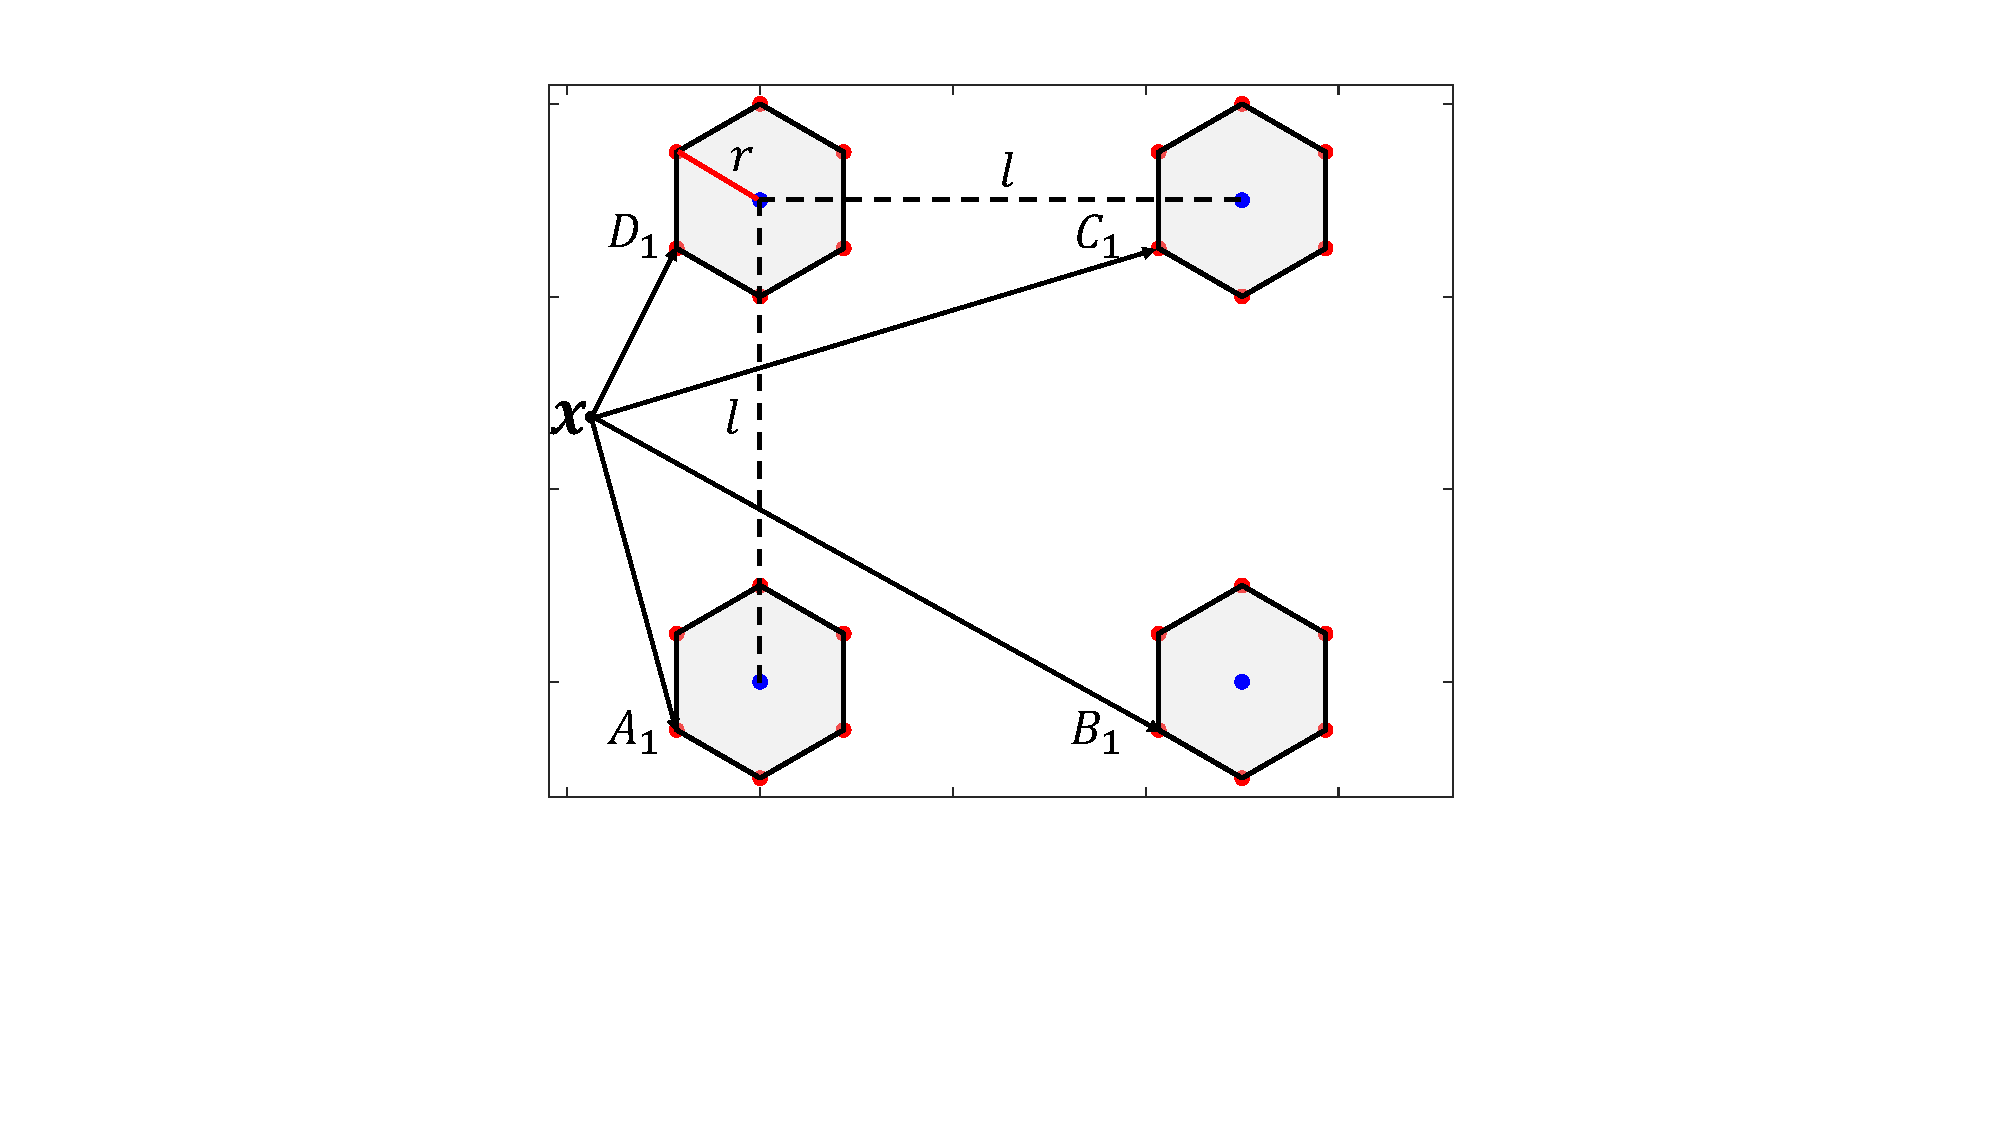
\includegraphics[width=.25\textwidth]{Section2/Problem}
	\caption{An example of Multi-Polygon test problem.}
	\label{fig:Multi-Polygon Problem}
\end{figure}

\subsection{Review of State-of-the-art Techniques}
\label{Review of State-of-the-art Techniques}
In this section, we provide a short review of state-of-the-art techniques for maintaining the diversity in the decision space. As pointed out by Deb \cite{Deb2001}, the key idea for solving MMOPs is to "divide" the entire population into several sub-populations that do not affect each other as much as possible, and then let each sub-population evolve independently. Here we list some commonly used approaches:
\subsubsection{Fitness Sharing Approach}
Fitness sharing was initially introduced in \cite{Goldberg} and widely adopted in MOEAs to keep the sparsity of the solutions in the objective space. The main idea of fitness sharing is to degrade the fitness of crowded solutions by sharing their fitness to their neighbors. In order to solve MMOPs, fitness sharing in both decision space and objective space needs to be considered simultaneously. For example, DNEA\cite{DNEA} uses two fitness sharing functions both in the decision and objective spaces. Fitness sharing approach is hard to apply because the sharing radius is a problem dependent parameter and it needs fine tuning. In addition, combining fitness sharing in two spaces is also a challenging task.
\subsubsection{Crowding Distance Approach}
Crowding distance is often used as a second selection criterion in Pareto-dominance based algorithms such as NSGA-II\cite{NSGA-II}. Several MMEAs such as Omni-optimizer\cite{Omni-Optimizer} and MO\_Ring\_PSO\_SCD\cite{MO-Ring-PSO-SCD} design special types of crowding distance that take both the decision and objective spaces into account.
\subsubsection{Restrict Environmental Selection Approach}
Carrying the environmental selection in the whole population is harmful to the population diversity in the decision space, which will be explained in Section \ref{Difficulties Analysis}. One remedy is to restrict the environmental selection in part of the population. More specifically, a solution should only compete with its neighborhood solutions in the decision space. The neighborhood relationship may either distance based or index based. For example, in MOEA/D-AD \cite{MOEA/D-AD}, a solution $\boldsymbol{x}$ only competes with the closest $L$ solutions in the decision space by the scalarizing function.

\section{Difficulties of Solving MMOPs}
\label{Difficulties Analysis}
Although there have been a lot of researches on MMOPs, the analysis of the difficulties of solving the MMOPs is still relatively rare. In this section, we analyze the difficulties of maintaining the diversity of the population in the decision space. Although most of the analysis is based on the Multi-polygon test problem, the result can be generalized to other MMOPs. 

At different stages of evolution, the reasons for affecting the distribution of population in the decision space may varies. We can use the IGD\cite{IGD} value to divide the evolutionary process into different phases. Suppose that the IGD values of the population at $t$ evaluations and the final population are $V_t$ and $V_f$ respectively. We define a relative error function $\delta_e(t)$:
$$\delta_e(t)=\frac{|V_t-V_f|}{V_f}$$
Then we can say that the population becomes mature at $T$ evaluations iff $\forall t<T$, $\delta_e(t)>\Delta$ and $\forall t \ge T$, $\delta(t) \leq \Delta$. Where $\Delta$ is a threshold defined by user. As shown in Fig. \ref{fig: Two stages}, the evolutionary process is separated into young and mature stages using $\Delta=3\%$.
\begin{figure}[htbp]
    \centering
    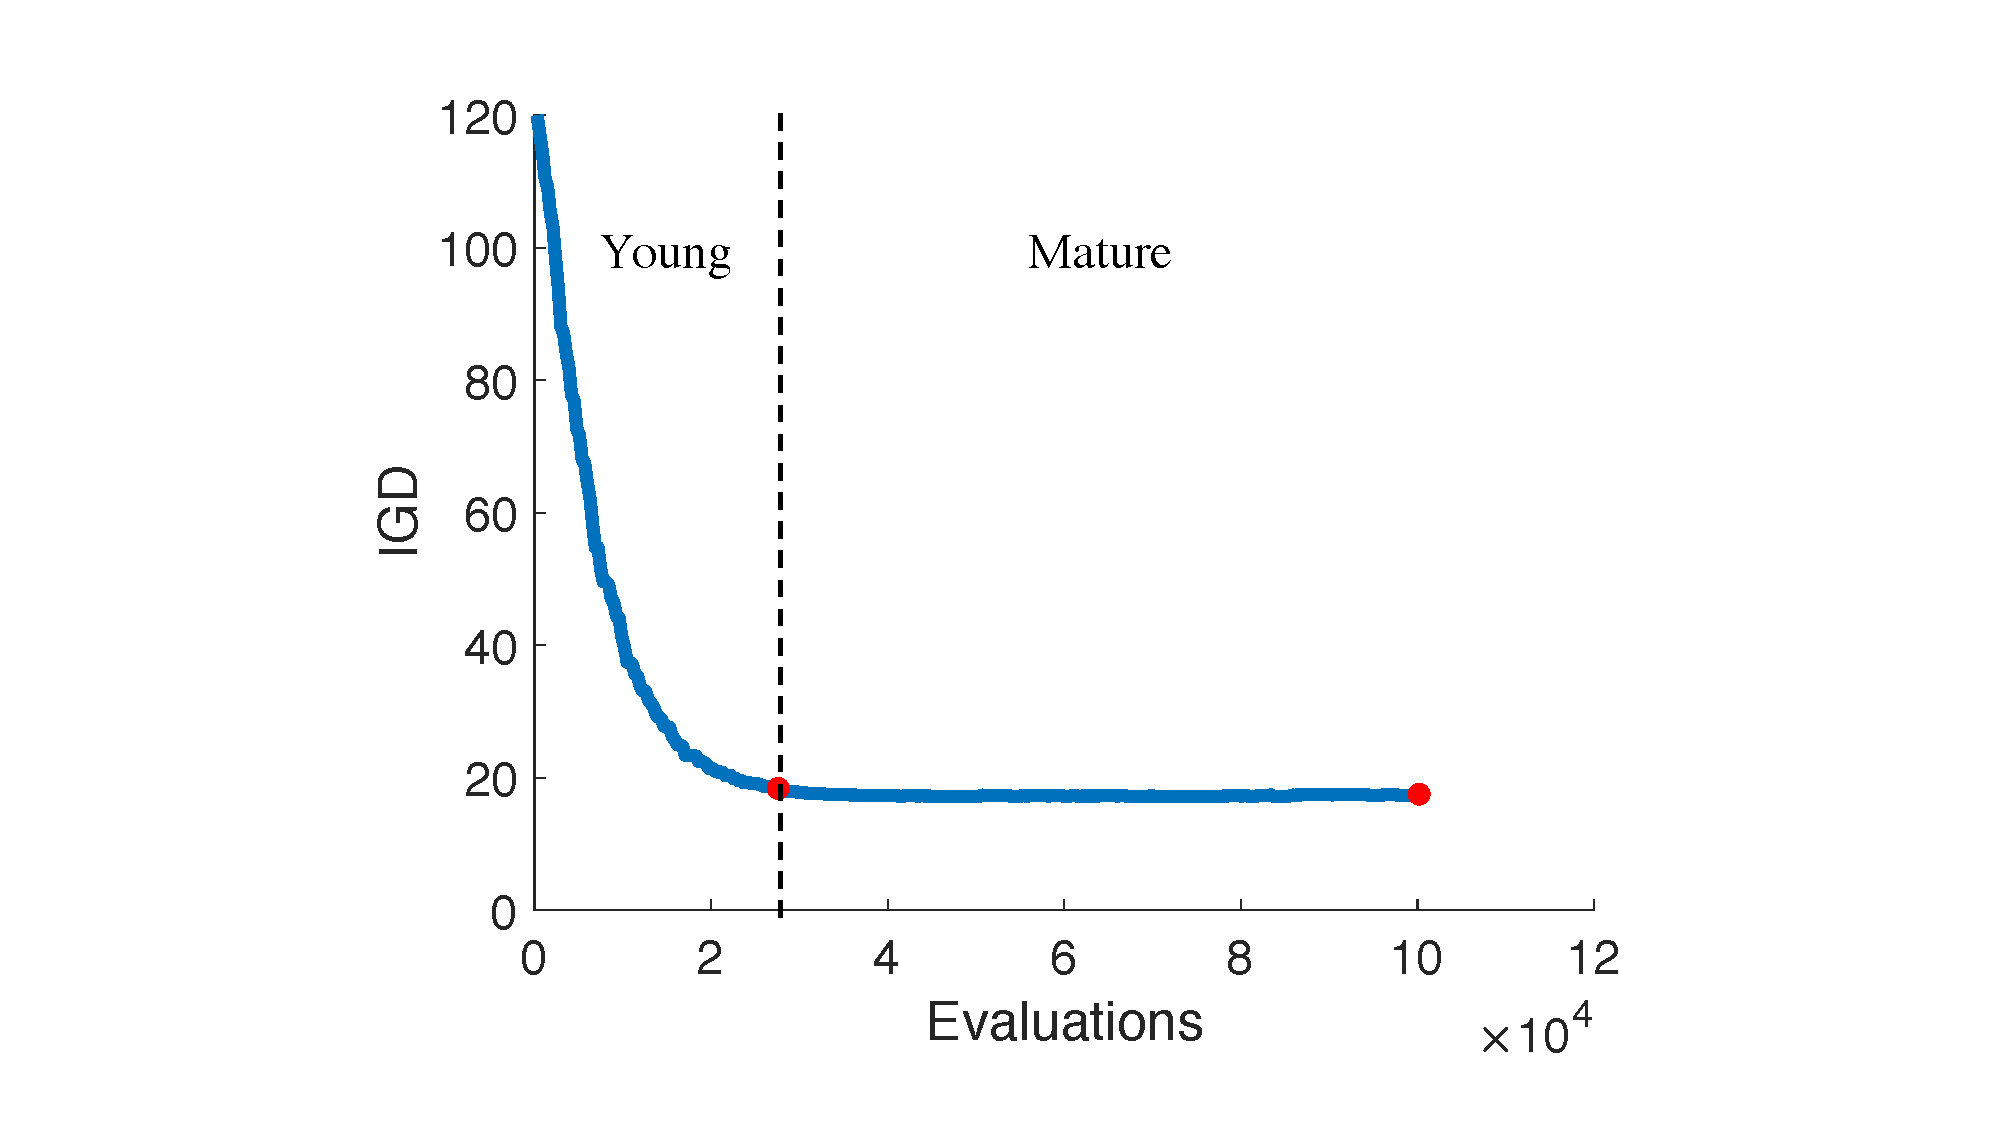
\includegraphics[width=.3\textwidth]{Section3/Stages}
    \caption{Two stages of evolution process.}
    \label{fig: Two stages}
\end{figure}

In the young stage, individuals in the population are far away from the PF. In the mature stage, the whole population is very close to the PF but the distribution of the population in the decision space may change. Now we analyze the difficulties for solving MMOPs from the following three aspects:

\subsection{Environmental Selection}
\label{Impact of environmental selection}
For most MOEAs, the environmental selection acts on the whole population. This will cause two consequences.
Firstly, in the young stage of the evolution, a relatively good solution will eliminate other dominated solutions which are far away from it in the decision space. Secondly, as pointed out in \cite{Liang2016}, for MMOPs, two solutions that are very far apart in the decision space may be very close in the objective space. Then MOEAs will remove the solutions that are too crowded in the objective space, therefore equivalent (or slightly inferior) solutions will be eliminated in the mature stage. As Fig. \ref{fig: Environmental selection} shows, for both cases, the diversity in the decision space will decrease. 

\begin{figure}[htbp]
	\centering
	\begin{subfigure}[b]{.24\textwidth}
		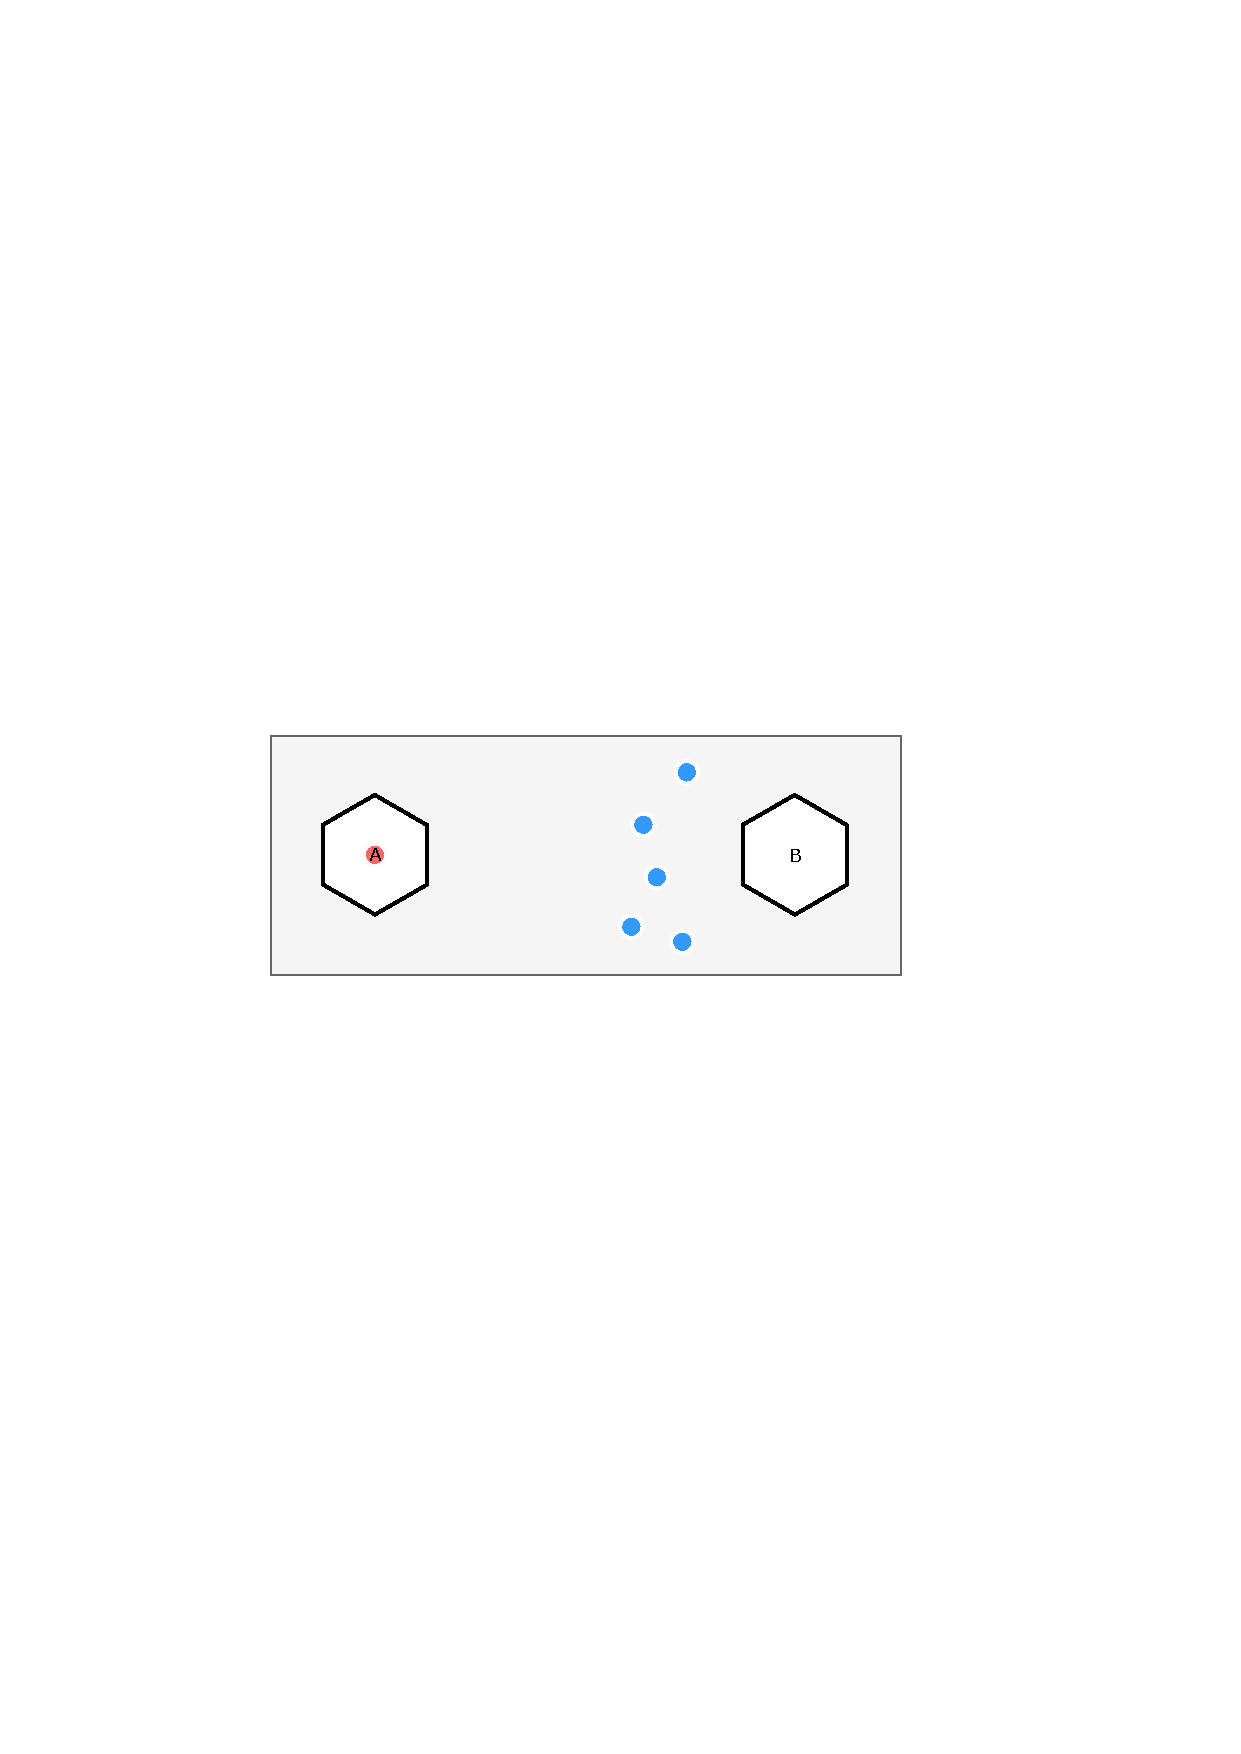
\includegraphics[width=\linewidth]{Section3/case1}
		\caption{Case 1}
	\end{subfigure}
	\begin{subfigure}[b]{.24\textwidth}
		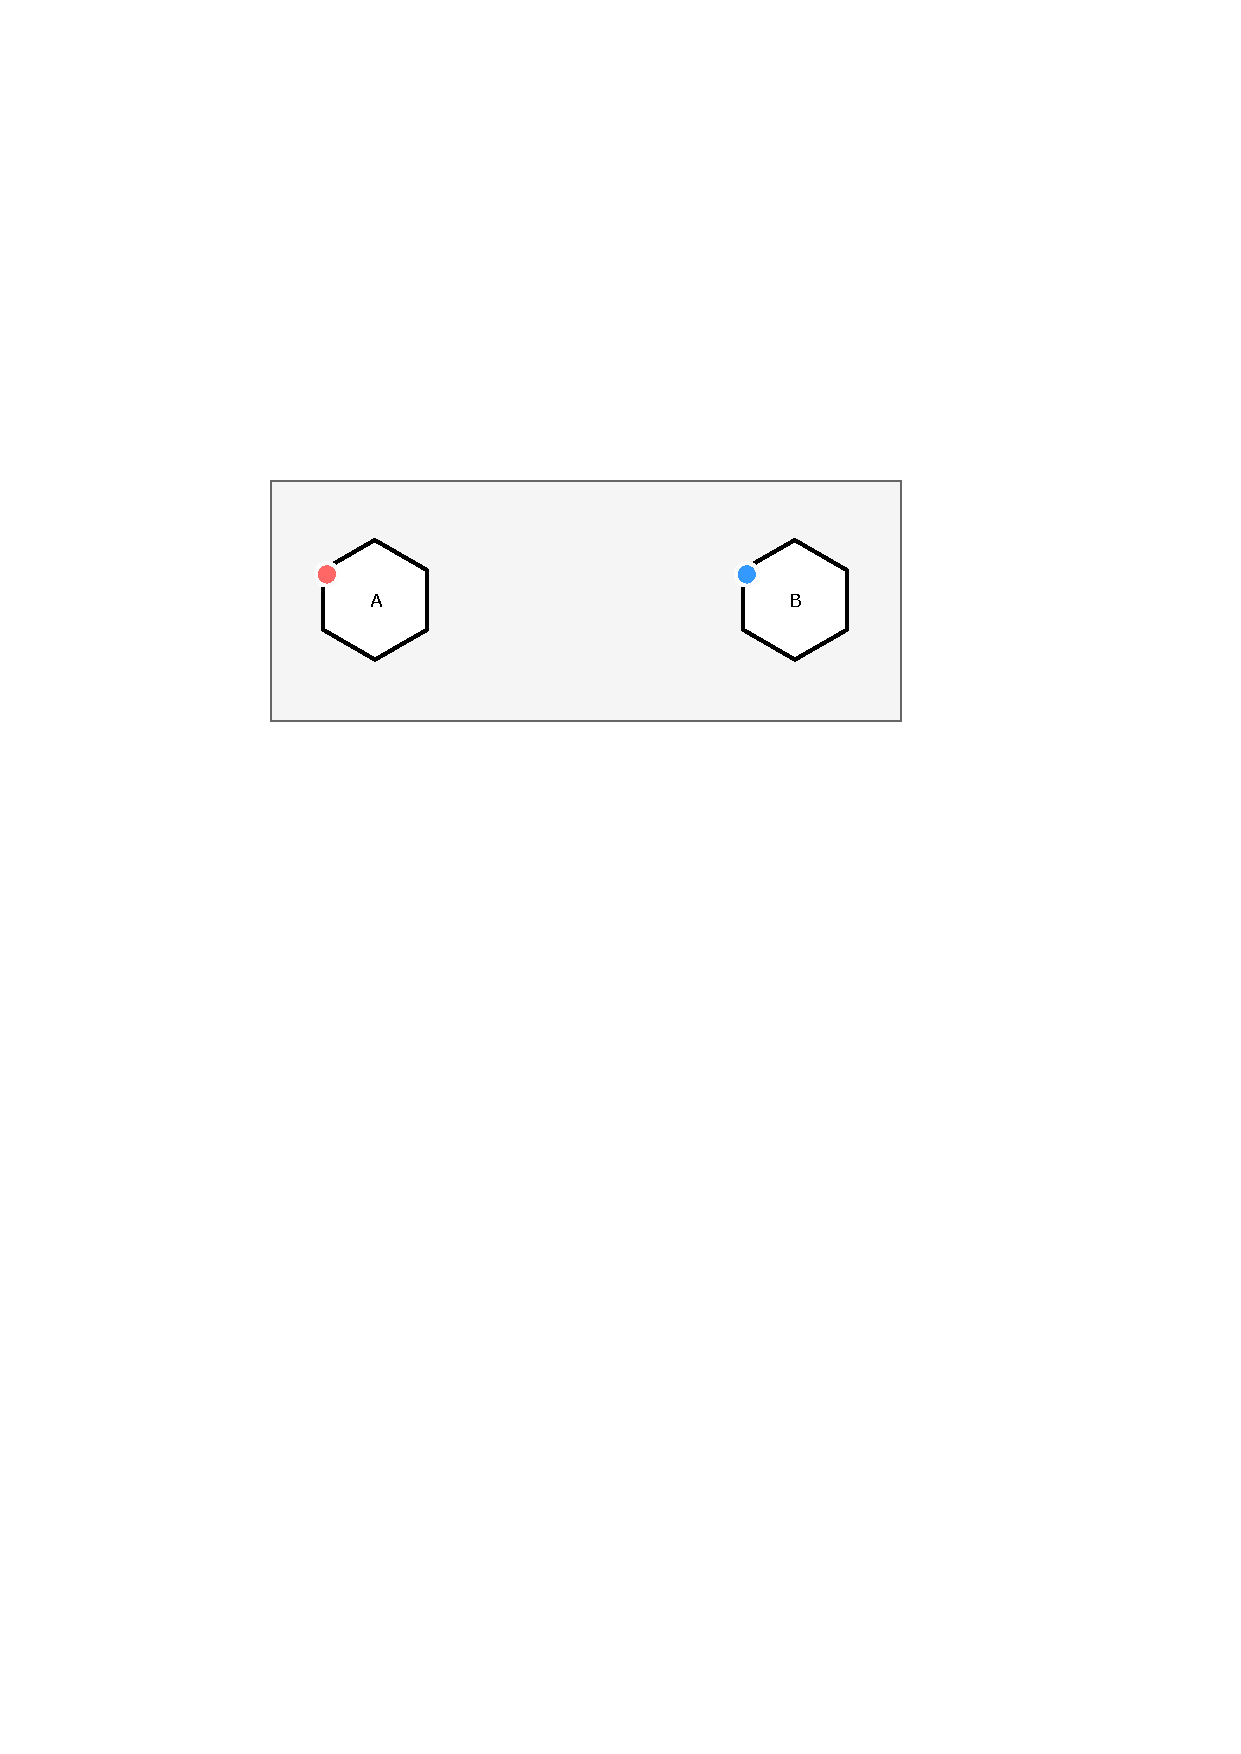
\includegraphics[width=\linewidth]{Section3/case2}
		\caption{Case 2}
	\end{subfigure}
	\caption{The impact of environmental selection on the diversity of the population in the decision space. In each case, only the red circle survive in the next generation.}
	\label{fig: Environmental selection}
\end{figure}


\subsection{Genetic Drift}
The reduction of the diversity in the decision space is also related to a concept called \textit{Genetic Drift}. Genetic drift is a phenomenon in which the frequency of alleles in a population declines due to random sampling errors \cite{GeneticDrift}. Fig. \ref{fig:Genetic drift demo} gives an example of genetic drift. At generation $t$, the population contains the same number of alleles $A$ and $a$, and we assume that only random sampling happens (no selection, mutation and crossover) from generation $t$ to $t+1$. Then the frequency of $A$ becomes larger than $a$ in generation $t+1$ due to the random sampling error. 

\begin{figure}[htbp]
	\centering
	\begin{subfigure}[b]{.24\textwidth}
		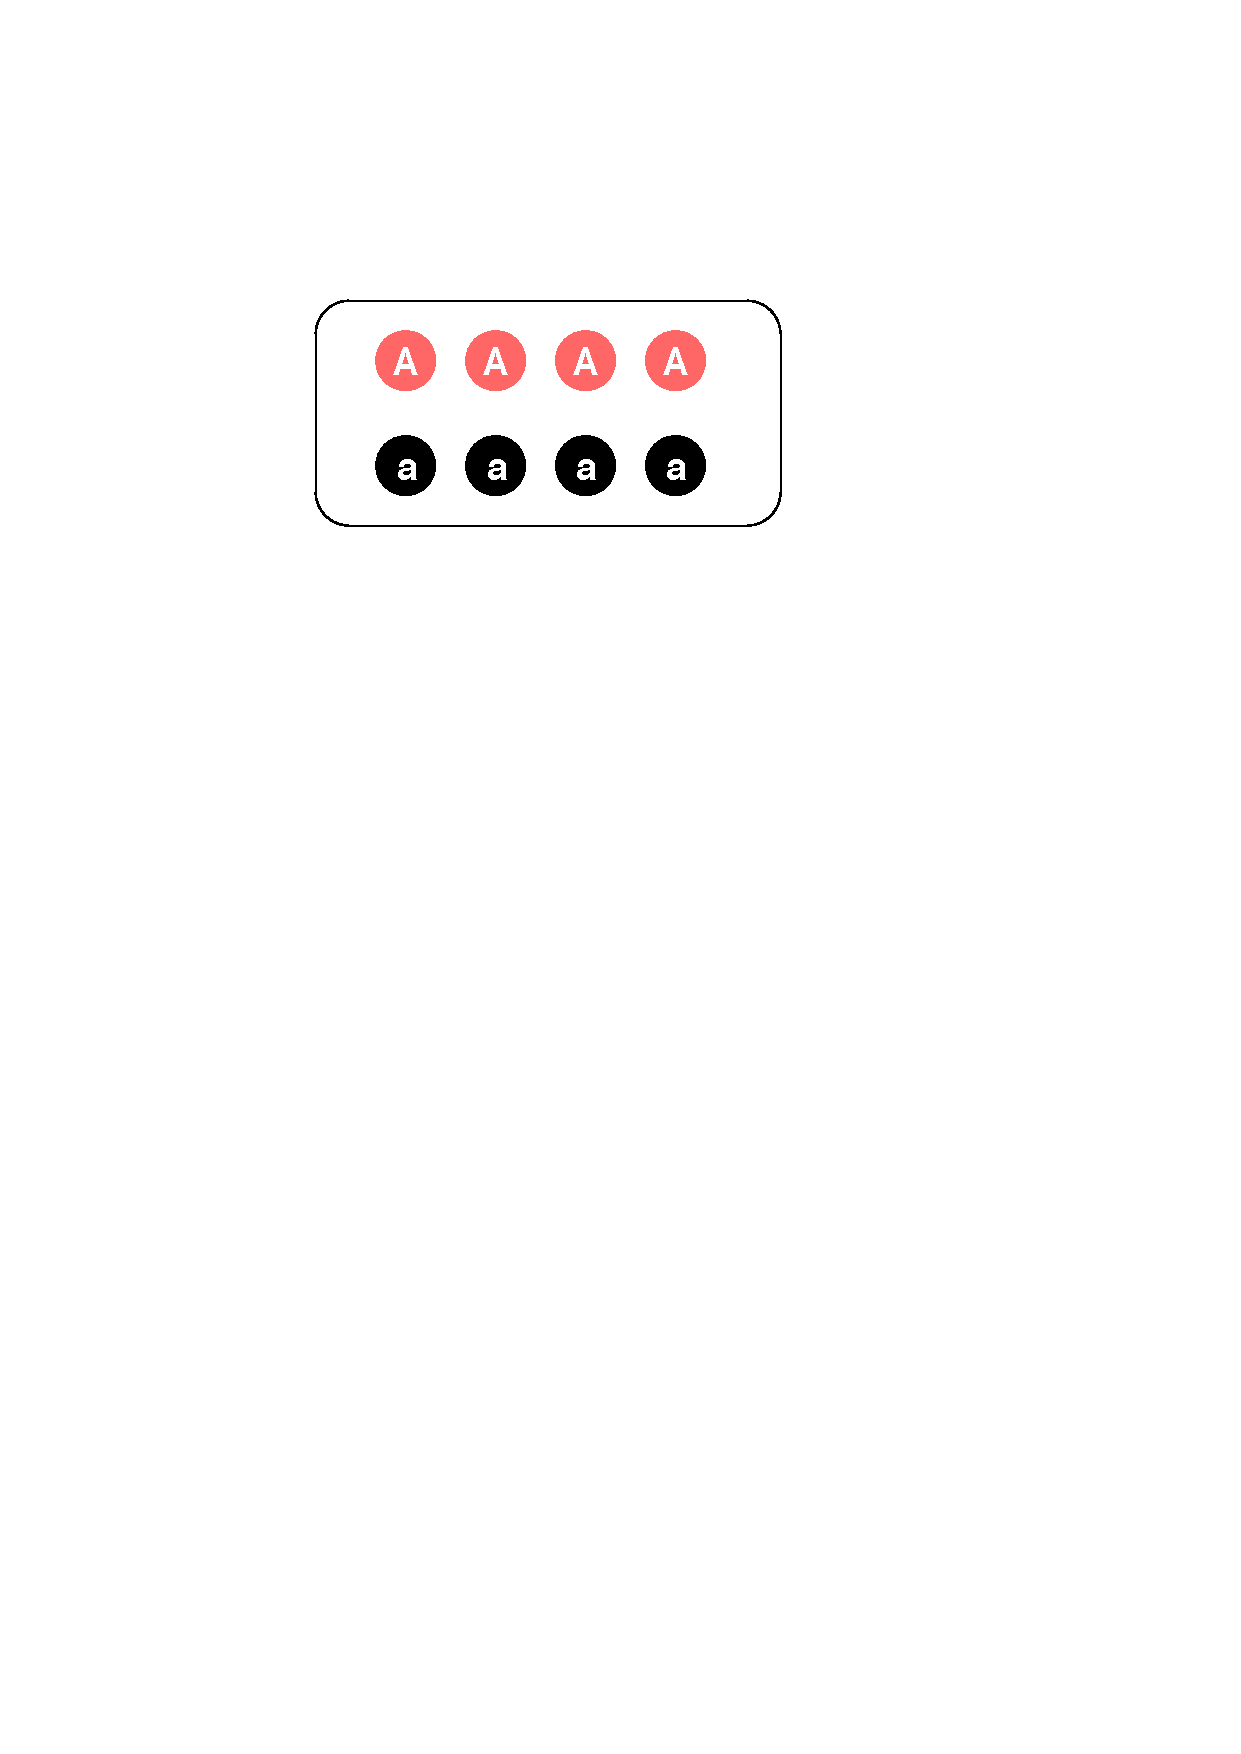
\includegraphics[width=\linewidth]{Section2/Generation_t}
		\caption{$freq_t(A) = freq_t(a)$}
	\end{subfigure}
	\begin{subfigure}[b]{.24\textwidth}
		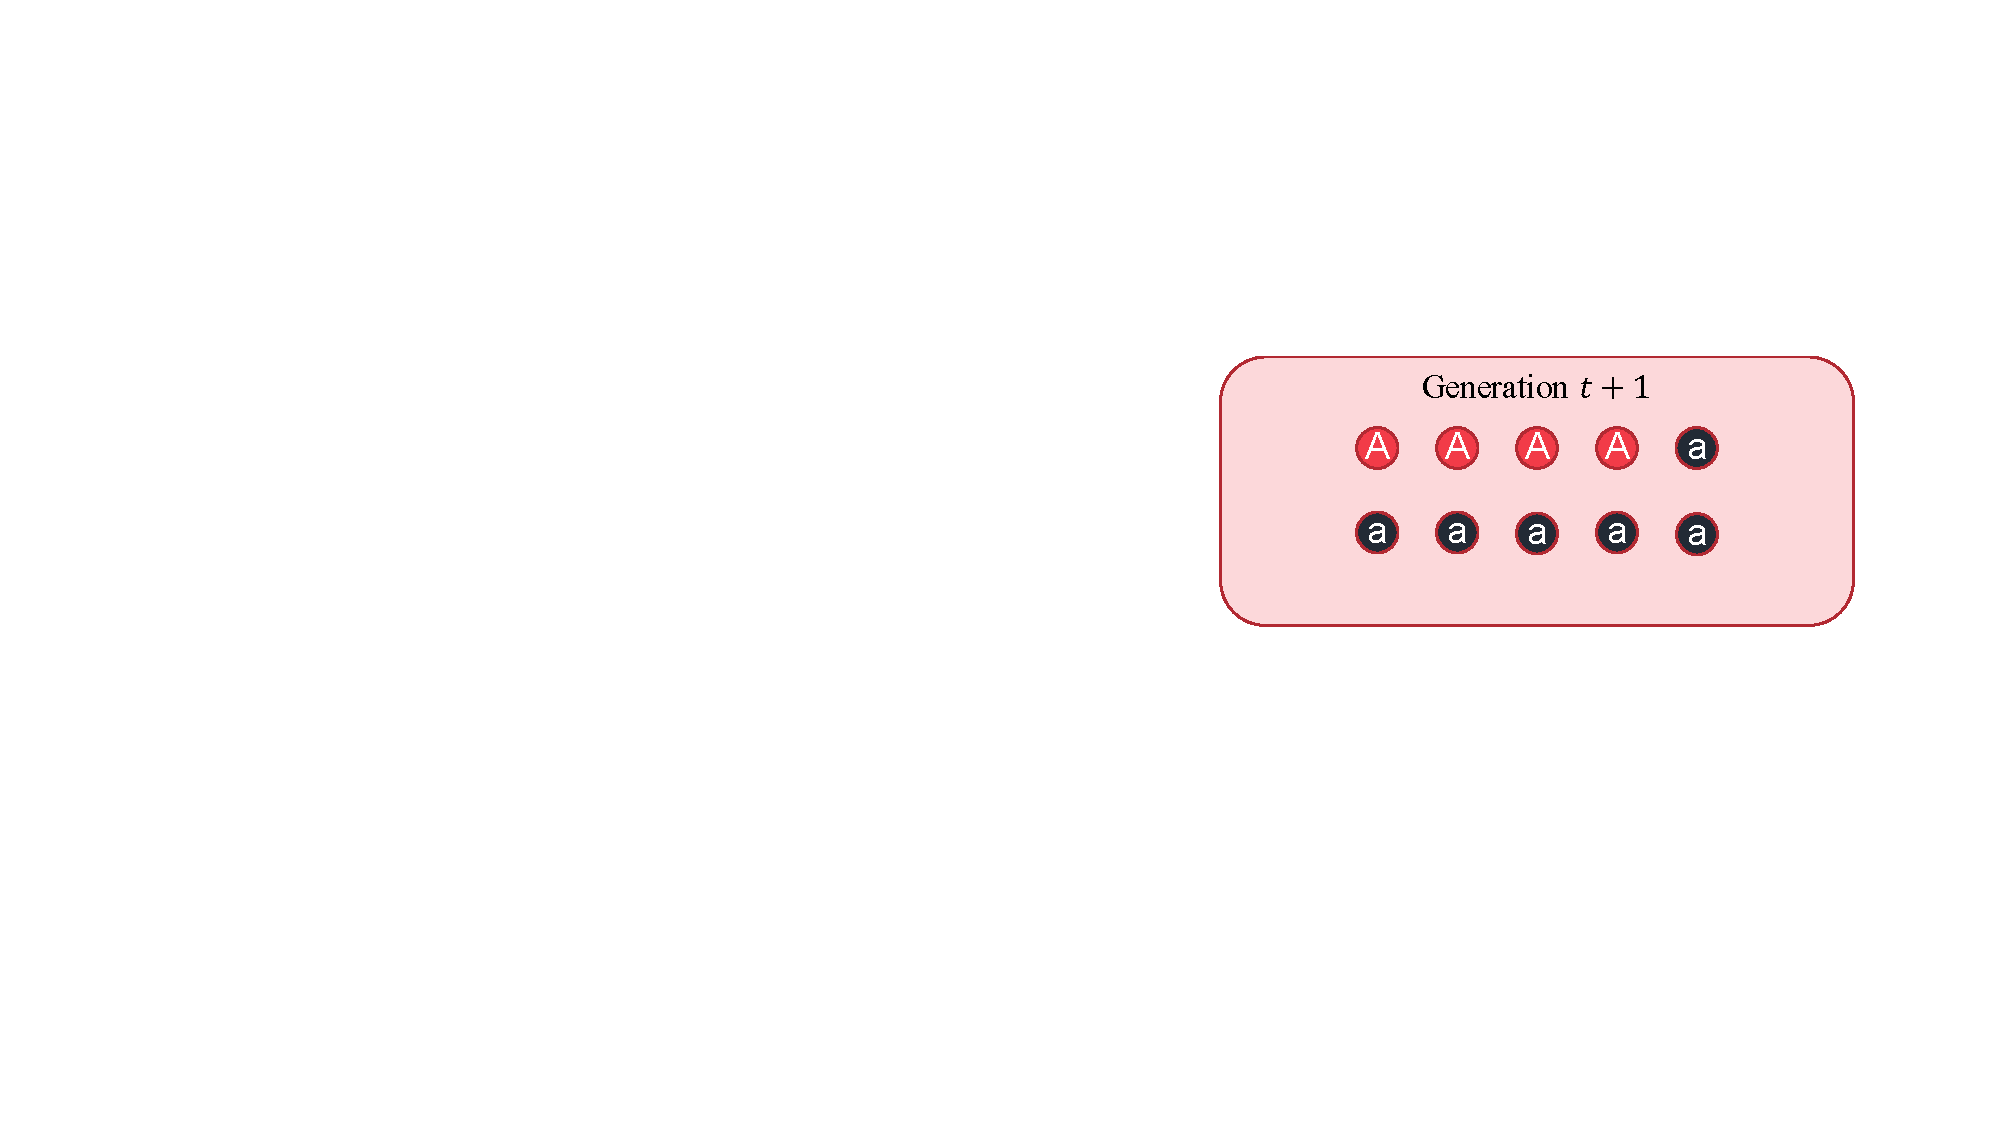
\includegraphics[width=\linewidth]{Section2/Generation_t1}
		\caption{$freq_{t+1}(A) < freq_{t+1}(a)$}
	\end{subfigure}
	\caption{Demonstration of genetic drift}
	\label{fig:Genetic drift demo}
\end{figure}

Genetic drift tends to reduce the genetic variation of the population during the evolutionary process. Some of the alleles may even disappear due to genetic drift. Asoh\cite{Asoh} mathematically proved that with only random selection, only one of alleles in the population will survive (this process is called convergence) as the iteration proceeds, and the mean convergence time is proportional to the population size. 

When solving MMOPs, equivalent solutions can be seen as alleles because they are indistinguishable in terms of objective function values. In Fig. \ref{fig: Alleles}, the decision space of Multi-Polygon test problem is divided into four parts. Solutions in each part can be viewed as an allele. Genetic drift can affect the distribution of the population in the decision space throughout the evolution process. In general, due to the existence of genetic drift, the diversity in the decision space will reduce. In section \ref{Experimental Studies}, we use more computational experiments to study the effects of genetic drift on solving MMOPs.

\begin{figure}[htbp]
    \centering
    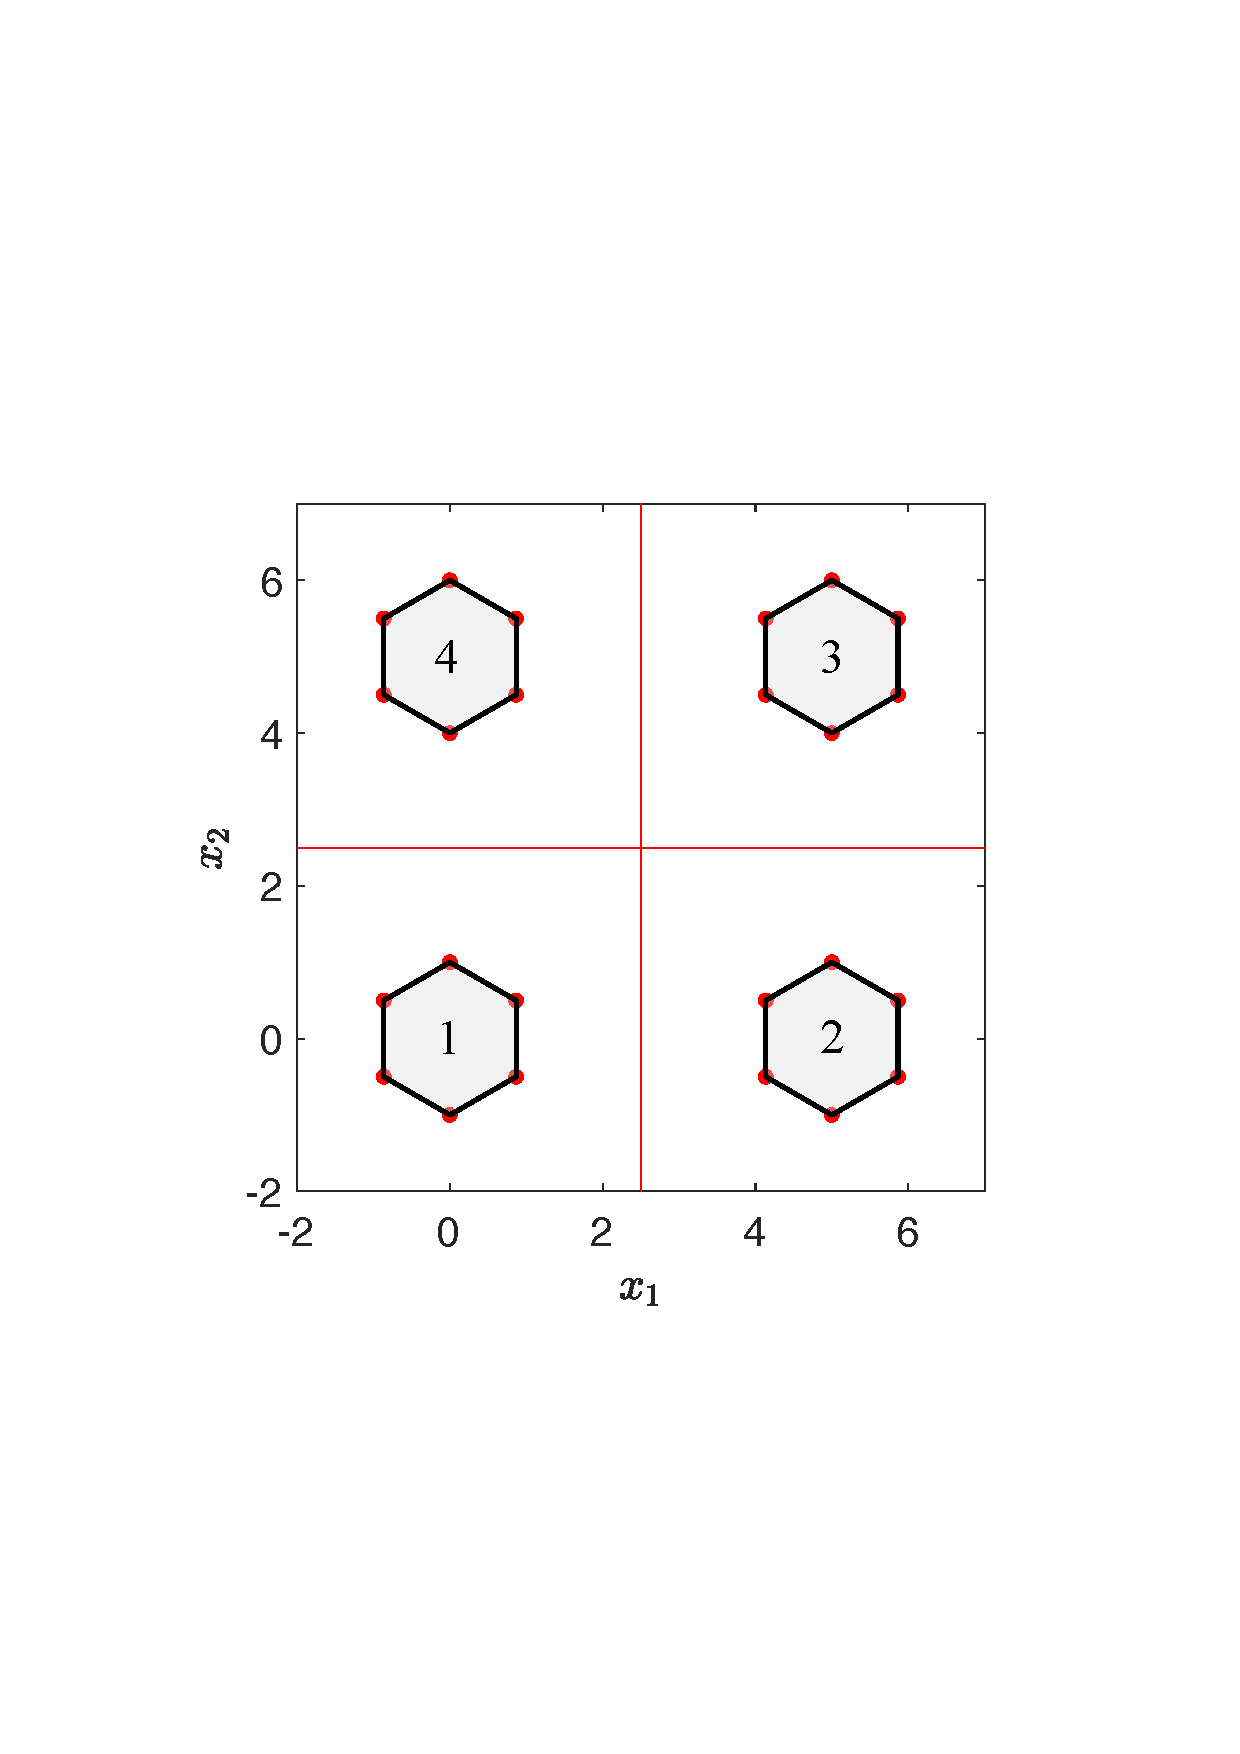
\includegraphics[width=.24\textwidth]{Section3/Alleles}
    \caption{Divide the decision space of Multi-Polygon test problem into 4 parts in counterclockwise order. Each part can be viewed as an gene allele.}
    \label{fig: Alleles}
\end{figure}

\subsection{Crossover and Mutation}
In evolutionary algorithms, crossover and mutation are two operations that will increase the variety of the population. These two operations can help the algorithm to avoid trapping in the local optima. However, since mutation and crossover have higher probability of producing offspring that are close to their parents, the distribution of the parent population will affect the distribution of the offspring population. More specifically, more offspring will be produced in the region where the parent population has higher density. Fig. \ref{fig: SBX crossover} demonstrates the results of generating 1,000 individuals from SBX\cite{SBX} with distribution index = 20. As shown in Fig. \ref{fig: SBX crossover} (\subref{fig: SBX crossover case 1}), the diversity of solutions in the decision space does not change too much since no new solutions are generated in other polygons. In Fig. \ref{fig: SBX crossover} (\subref{fig: SBX crossover case 2}), the parents are two solutions in diagonal polygons, i.e. $(0, 0)^T$ and $(5, 5)^T$. In this case, the diversity of solutions in the decision space increases dramatically since the number of alleles in the population increases from two to four. Fig. \ref{fig: Polynomial mutation} depicts the results of polynomial mutation with distribution index = 20. The number of alleles is not changed by mutation. From these two simulation results, we can see that traditional crossover and mutation operations may not be able to effectively increase the diversity in the decision space.
\begin{figure}[htbp]
	\centering
	\begin{subfigure}[b]{.24\textwidth}
		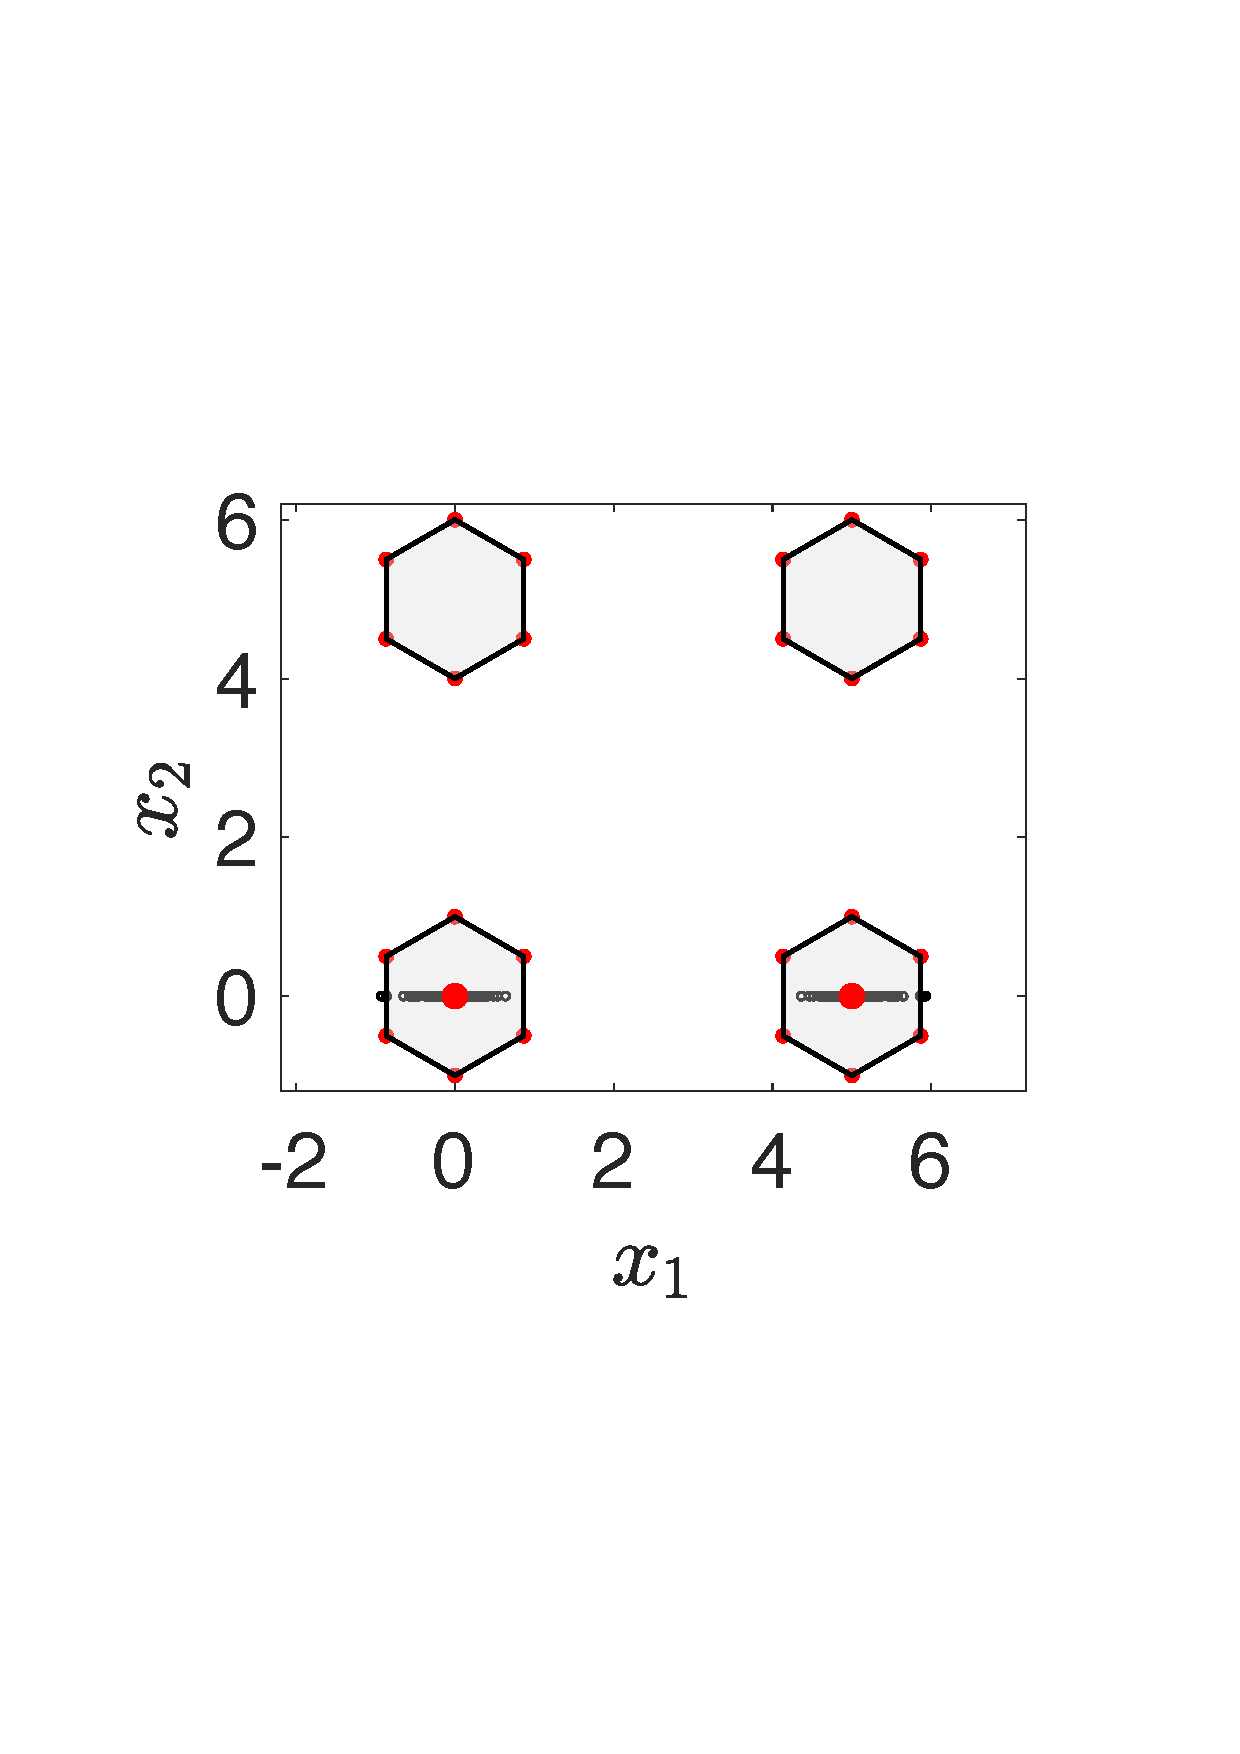
\includegraphics[width=\linewidth]{Section3/crossover1}
		\caption{Case 1: parents are $(0, 0)^T$ and $(5, 0)^T$. The number of alleles remains unchanged.}
		\label{fig: SBX crossover case 1}
	\end{subfigure}
	\begin{subfigure}[b]{.24\textwidth}
		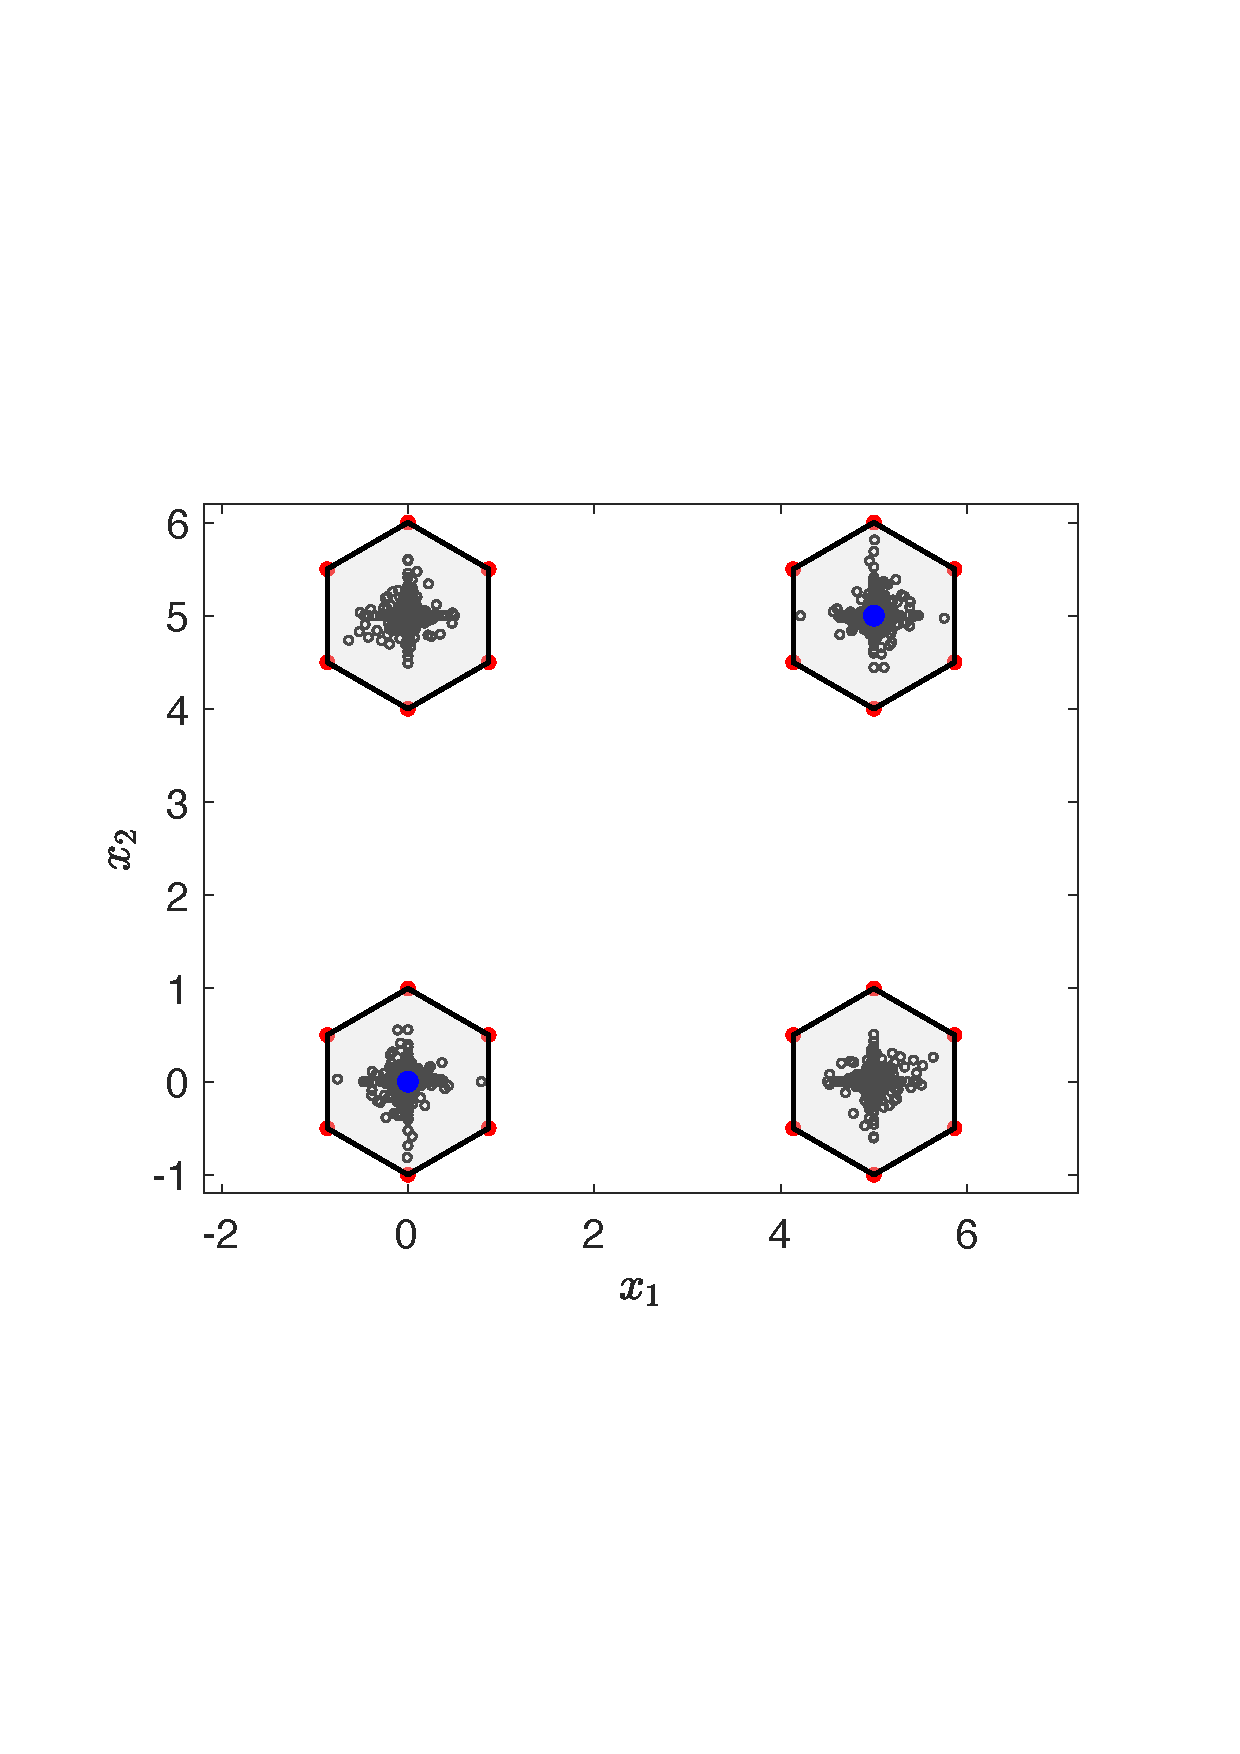
\includegraphics[width=\linewidth]{Section3/crossover2}
		\caption{Case 2: parents are $(0, 0)^T$ and $(5, 5)^T$. The number of alleles changes from 2 to 4.}
		\label{fig: SBX crossover case 2}
	\end{subfigure}
	\caption{Generate 1,000 offspring by SBX crossover. Yellow and dark circles represent parent and offspring respectively.}
	\label{fig: SBX crossover}
\end{figure}

\begin{figure}[htbp]
    \centering
    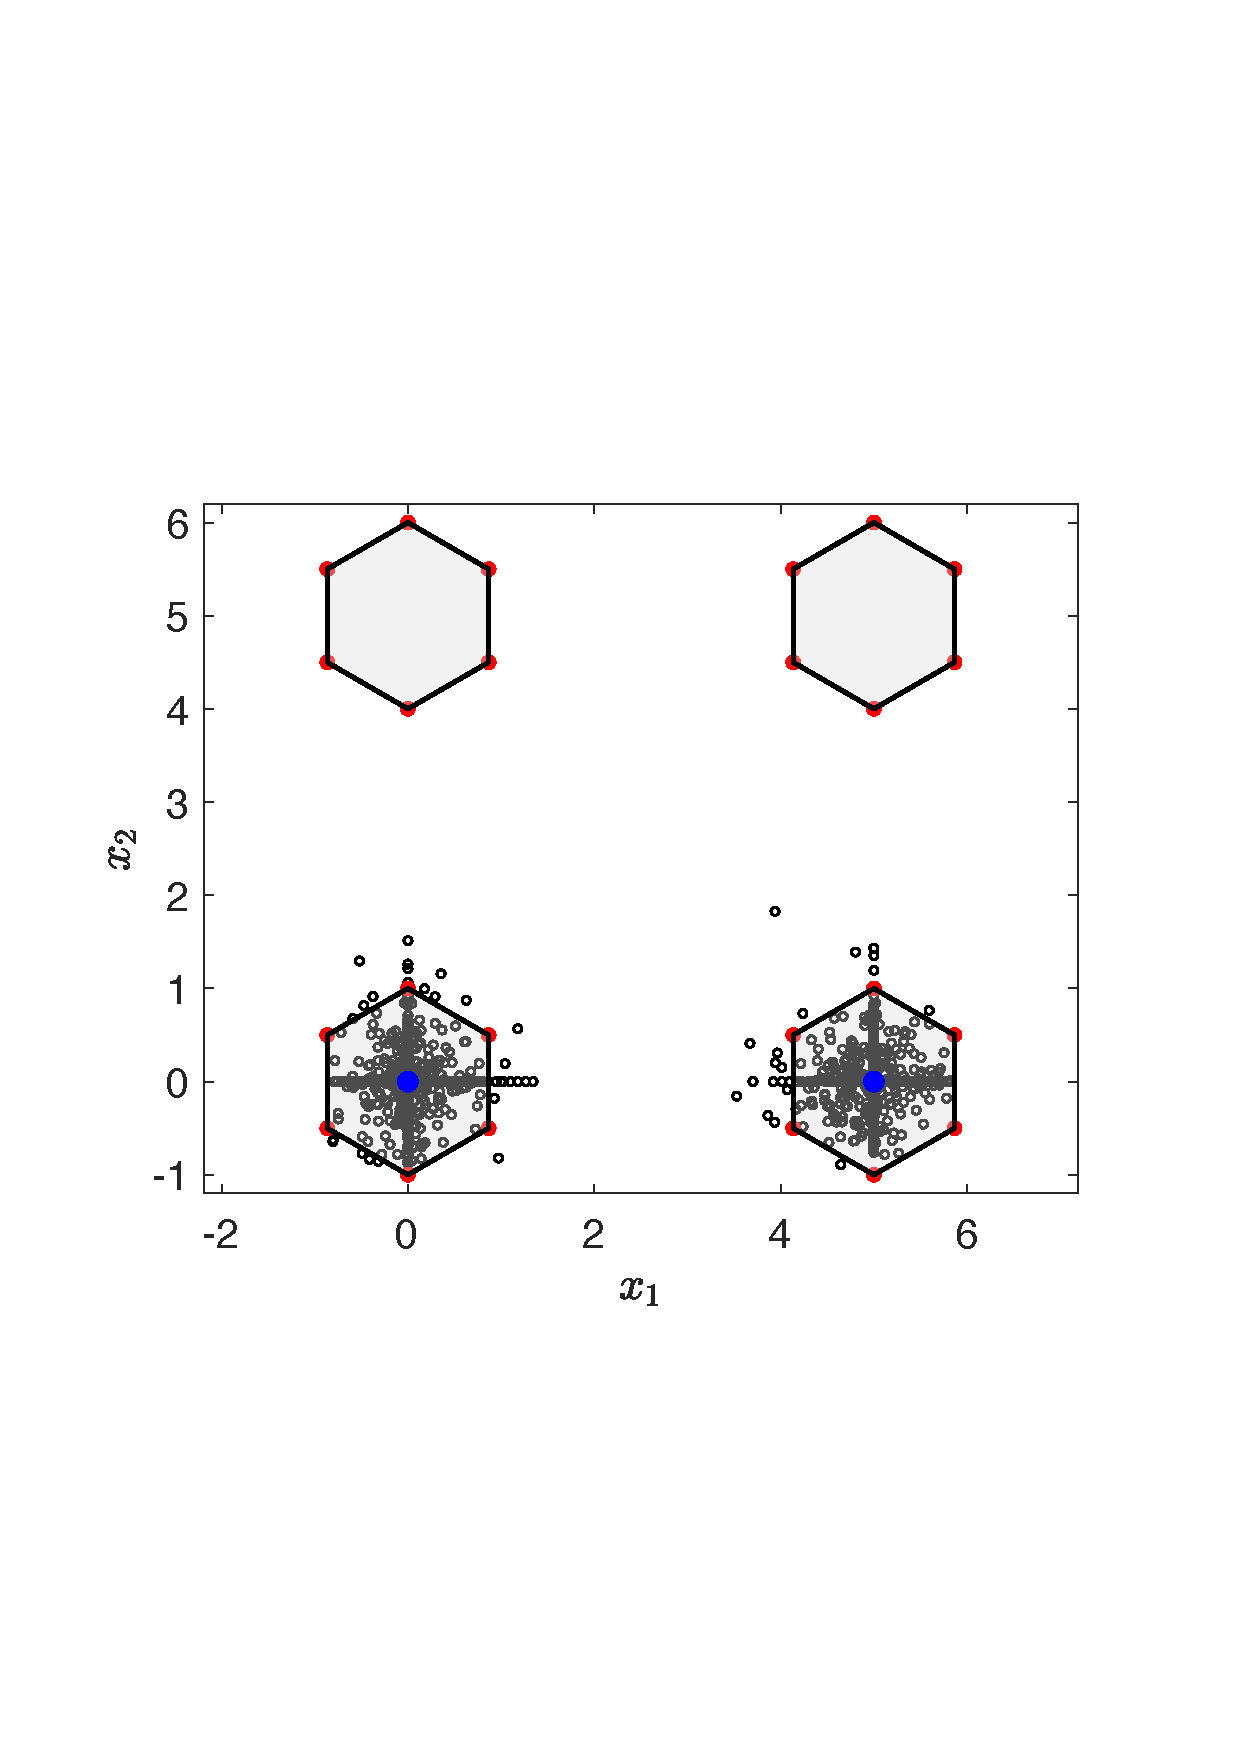
\includegraphics[width=.24\textwidth]{Section3/mutation}
    \caption{Generate 1,000 offspring by applying polynomial mutation to two solutions. Yellow and dark circles represent parent and offspring respectively. The number of alleles remains unchanged.}
    \label{fig: Polynomial mutation}
\end{figure}
From the discussion above, we can see that extra diversity maintenance techniques are necessary to maintain the diversity of the population in the decision space.

\section{Experimental Studies}
\label{Experimental Studies}
\subsection{Experimental Settings}
\label{Experimental Settings}
\subsubsection{Algorithms for Comparison}
In order to obtain more reliable experimental results, we select several representative MOEAs from the following three classes:
\begin{itemize}
    \item \textbf{Pareto-dominance based}: NSGA-II\cite{NSGA-II}, NSGA-III\cite{NSGA-III} and SPEA2\cite{SPEA2}.
    \item \textbf{Decomposition based}: MOEA/D \cite{MOEA/D} with PBI($\theta=5$) and Tchebycheff aggregation function.
    \item \textbf{Indicator based}: IBEA\cite{IBEA}.
\end{itemize}

Also, for MMEAs, we selected algorithms mentioned in section \ref{Review of State-of-the-art Techniques}: DNEA, MO\_Ring\_PSO\_SCD, MOEA/D-AD and Omni-Optimizer.
\subsubsection{Parameter Settings}
In our experiments, we use the following parameter settings: 
\paragraph{Test Problem Settings}
\begin{itemize}
     \item Number of objectives $M=6$.
    \item Number of decision variables $D=2, 4, 6, 8, 10, 100$.
    \item Four regular polygons with radius $r=1$ and their centers are $\boldsymbol{c}_1=(0, 0)^T$, $\boldsymbol{c}_2=(5, 0)^T$, $\boldsymbol{c}_3=(5, 5)^T$, $\boldsymbol{c}_4=(0, 5)^T$. 
\end{itemize}
\paragraph{GA Settings}
\begin{itemize}
    \item Population size $N$ = 300.
    \item Number of evaluations = $10^5$.
    \item SBX crossover(distribution index = 20) with probability 1.0.
    \item Polynomial mutation(distribution index = 20) with probability $1/D$.
\end{itemize}
\paragraph{Algorithm Settings}
We use default parameters for each algorithm according to the corresponding papers.
\begin{itemize}
    \item IBEA: fitness scaling factor $\kappa=0.05$.
    \item DNEA: niche radius in the objective space $\delta_{obj}=0.06$ and niche radius in the decision space $\delta_{var}=0.02$.
    \item MO\_Ring\_PSO\_SCD: the size of personal best archive $n_{\text{PBA}}=5$ and the size of neighborhood best archive $n_{\text{NBA}}=15$.
    \item MOEA/D-AD: use PBI($\theta=5$) aggregation function and neighborhood size $L = \lfloor 0.1\mu \rfloor$ where $\mu$ is the size of current population.
    \item Omni-optimizer: $\epsilon$-dominance parameter $\delta=0.001$.
\end{itemize}

\subsection{Experimental Results and Analysis}
\label{Experimental Results}
In this section, we evaluate the performance of the selected MOEAs and MMEAs on Multi-Polygon test problems with different dimensional decision spaces using PlatEMO platform\cite{PlatEMO}. In each experiment, each algorithm runs 31 times and the run with median HV among them is reported. In addition, following the similar manner from paper \cite{Hisao}, we plot the 2-d projection of the obtained solutions to visualize their distribution in the decision space. Furthermore, we compare the performance of MOEAs and MMEAs in the objective space.
%% dim = 2 PS plot 
\begin{figure}[htbp]
    \centering
    \begin{subfigure}[b]{.24\textwidth}
    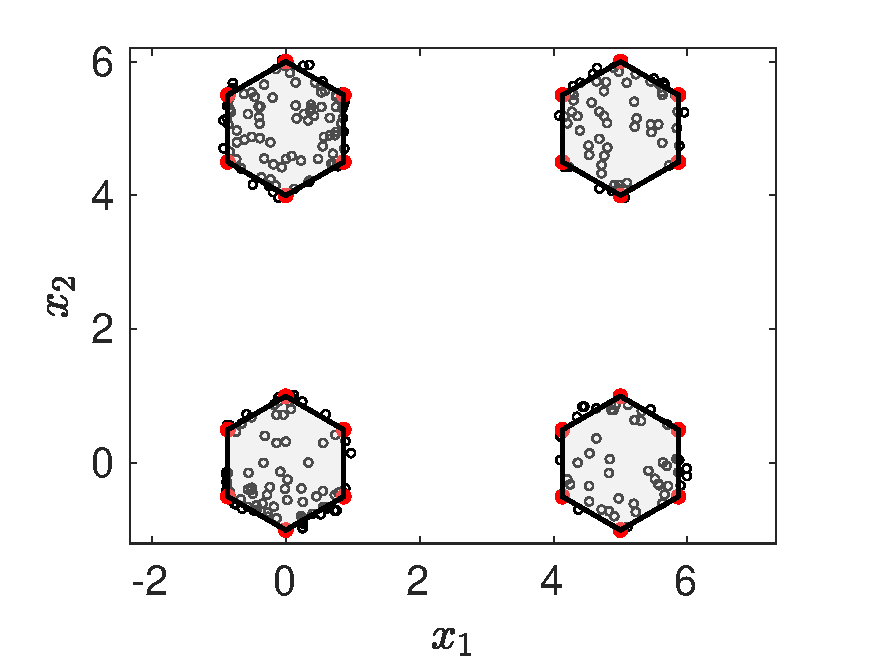
\includegraphics[width=\linewidth]{Section5/dim2/PS/NSGAII}
    \caption{NSGA-II}
    \end{subfigure}
    \begin{subfigure}[b]{.24\textwidth}
    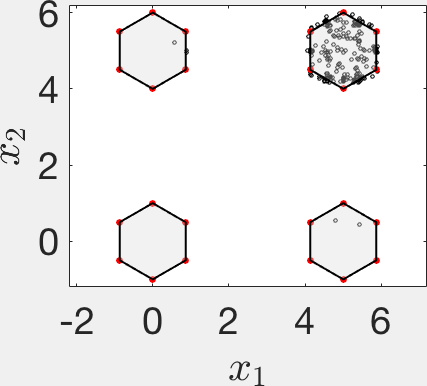
\includegraphics[width=\linewidth]{Section5/dim2/PS/NSGAIII}
    \caption{NSGA-III}
    \end{subfigure}
    
    \begin{subfigure}[b]{.24\textwidth}
    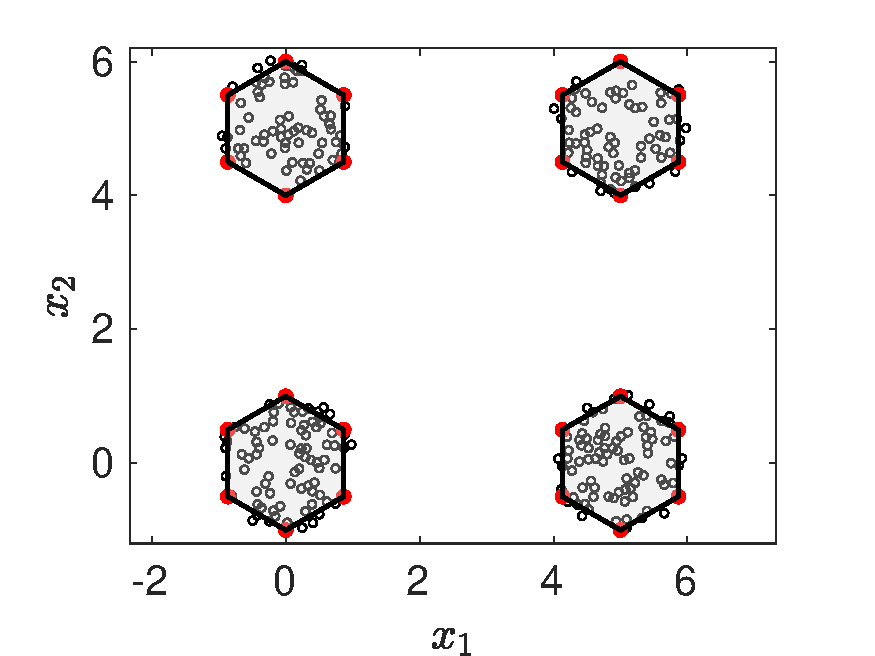
\includegraphics[width=\linewidth]{Section5/dim2/PS/SPEA2}
    \caption{SPEA2}
    \end{subfigure}
    \begin{subfigure}[b]{.24\textwidth}
    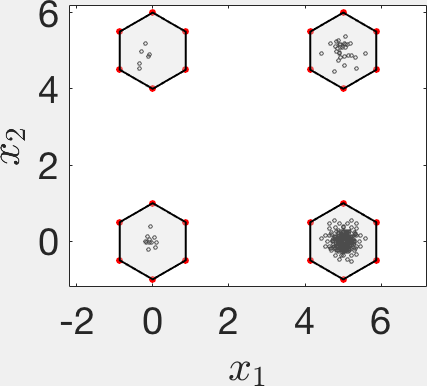
\includegraphics[width=\linewidth]{Section5/dim2/PS/MOEAD_TCH}
    \caption{MOEA/D-TCH}
    \end{subfigure}
    
    \begin{subfigure}[b]{.24\textwidth}
    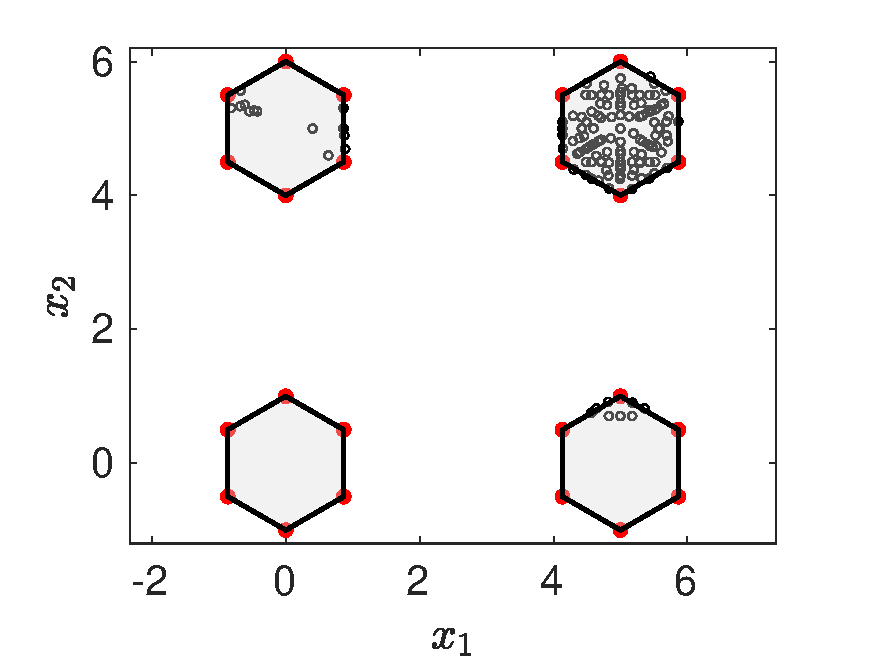
\includegraphics[width=\linewidth]{Section5/dim2/PS/MOEAD_PBI}
    \caption{MOEA/D-PBI}
    \end{subfigure}
    \begin{subfigure}[b]{.24\textwidth}
    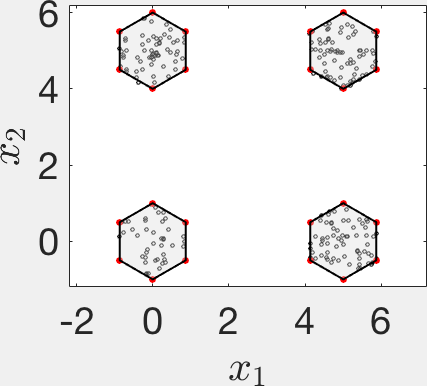
\includegraphics[width=\linewidth]{Section5/dim2/PS/IBEA}
    \caption{IBEA}
    \end{subfigure}

    \caption{Simulation results of MOEAs on Multi-Polygon test problem with $D=2$.}
    \label{fig: MOEAs PS dim=2}
\end{figure}

\begin{figure}[htbp]
    \centering
    \begin{subfigure}[b]{.24\textwidth}
    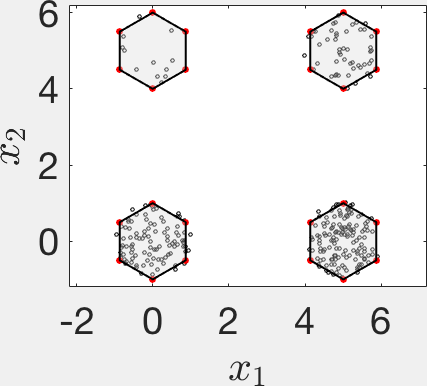
\includegraphics[width=\linewidth]{Section5/dim2/PS/DNEA}
    \caption{DNEA}
    \end{subfigure}
    \begin{subfigure}[b]{.24\textwidth}
    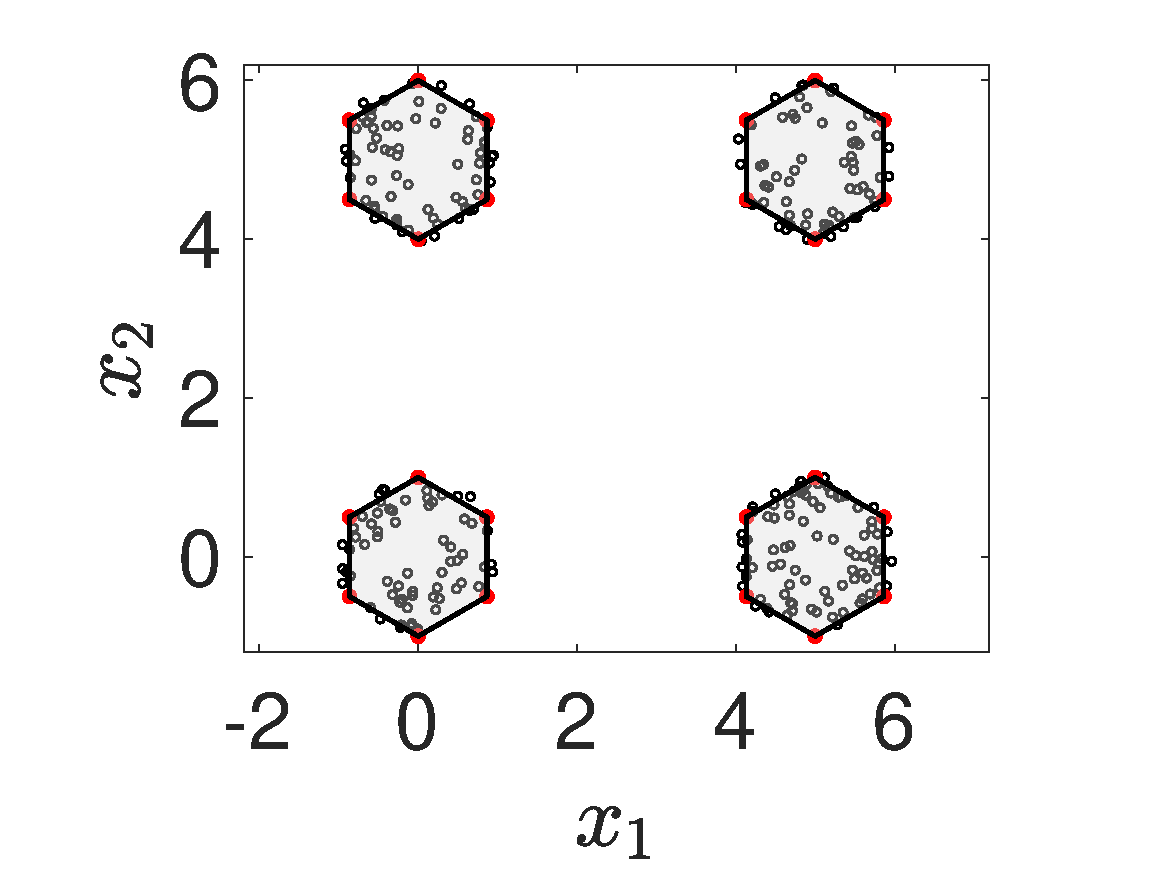
\includegraphics[width=\linewidth]{Section5/dim2/PS/MO_Ring_PSO_SCD}
    \caption{MO\_Ring\_PSO\_SCD}
    \end{subfigure}
    
    \begin{subfigure}[b]{.24\textwidth}
    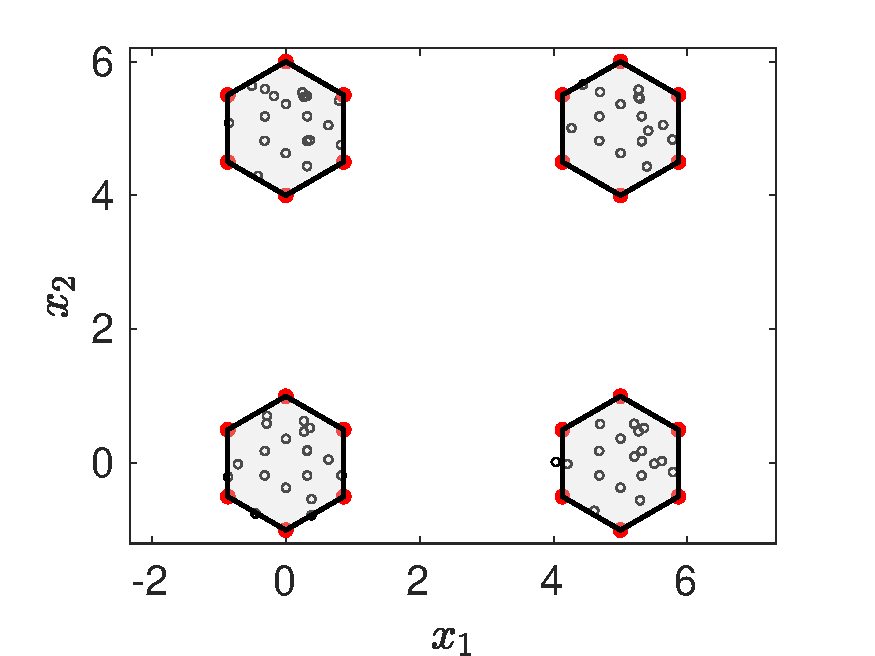
\includegraphics[width=\linewidth]{Section5/dim2/PS/MOEADAD}
    \caption{MOEA/D-AD}
    \end{subfigure}
    \begin{subfigure}[b]{.24\textwidth}
    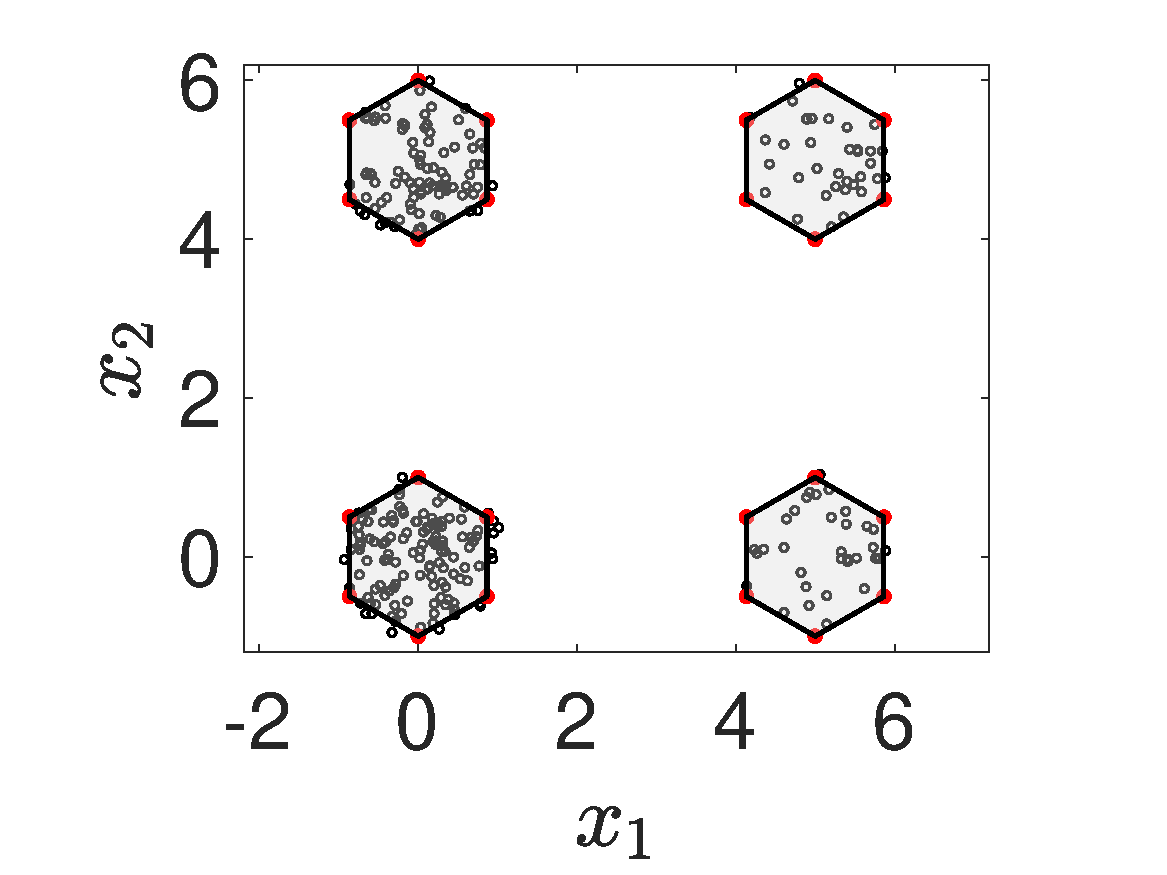
\includegraphics[width=\linewidth]{Section5/dim2/PS/OmniOptimizer}
    \caption{Omni-optimizer}
    \end{subfigure}
    \caption{Simulation results of MMEAs on Multi-Polygon test problem with $D=2$.}
    \label{fig: MMEAs PS dim=2}
\end{figure}

Figs. \ref{fig: MOEAs PS dim=2} and \ref{fig: MMEAs PS dim=2} show the simulation results of MOEAs and MMEAs when $D=2$. It can be seen that the performance of MOEA/D and NSGA-III is worse than other algorithms. When $D=2$, all algorithms except MOEA/D and NSGA-III can obtain a good coverage of the true Pareto sets. It is worth mentioning that, the number of solutions obtained by MOEA/D-AD is smaller than others due to the deletion mechanism.

As discussed in section \ref{Difficulties Analysis}, we pointed out that the performance of MOEAs on the MMOPs should be very poor. However, the experimental results here are inconsistent with this proposition. In order to figure out the reason, we divide the plane into four parts, and mark them as area 1\textasciitilde 4 in counterclockwise order as shown in Fig. \ref{fig: Alleles}. Then, after every 500 evaluations (denoted as epoch), the number of solutions in each area is recorded. In addition, the IGD value of each epoch is also recorded to show the evolutionary progress. 

%% dim = 2 Diversity Plot
\begin{figure}[htbp]
    \centering
    \begin{subfigure}[b]{.24\textwidth}
    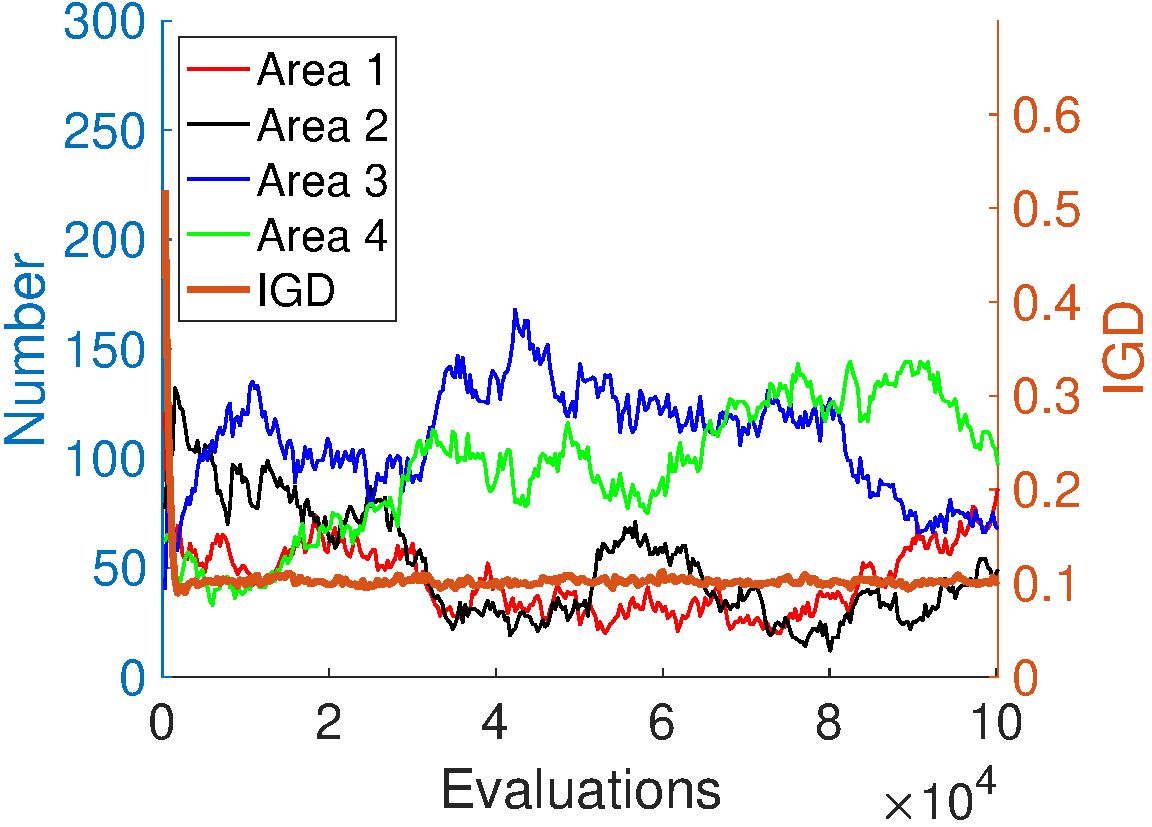
\includegraphics[width=\linewidth]{Section5/dim2/Diversity/NSGAII}
    \caption{NSGA-II}
    \end{subfigure}
    \begin{subfigure}[b]{.24\textwidth}
    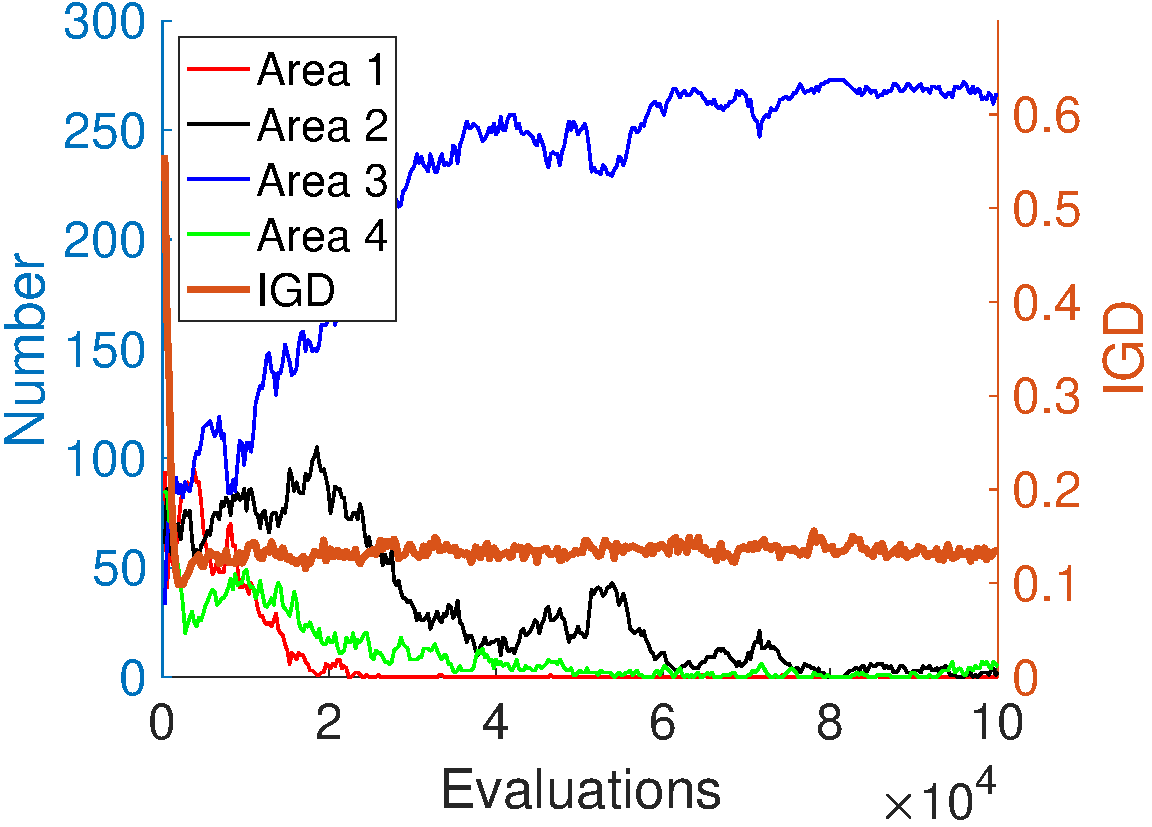
\includegraphics[width=\linewidth]{Section5/dim2/Diversity/NSGAIII}
    \caption{NSGA-III}
    \label{fig: NSGA-III Diversity dim=2}
    
    \end{subfigure}
    \begin{subfigure}[b]{.24\textwidth}
    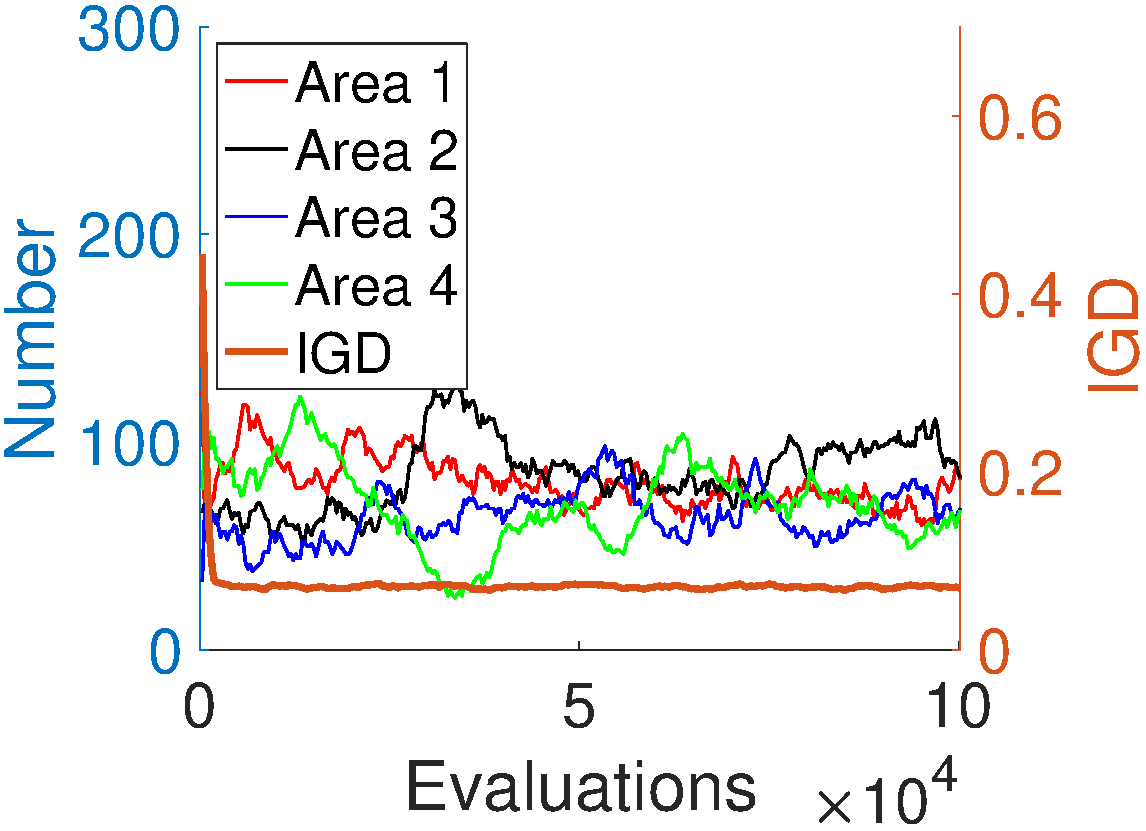
\includegraphics[width=\linewidth]{Section5/dim2/Diversity/SPEA2}
    \caption{SPEA2}
    \end{subfigure}
    \begin{subfigure}[b]{.24\textwidth}
    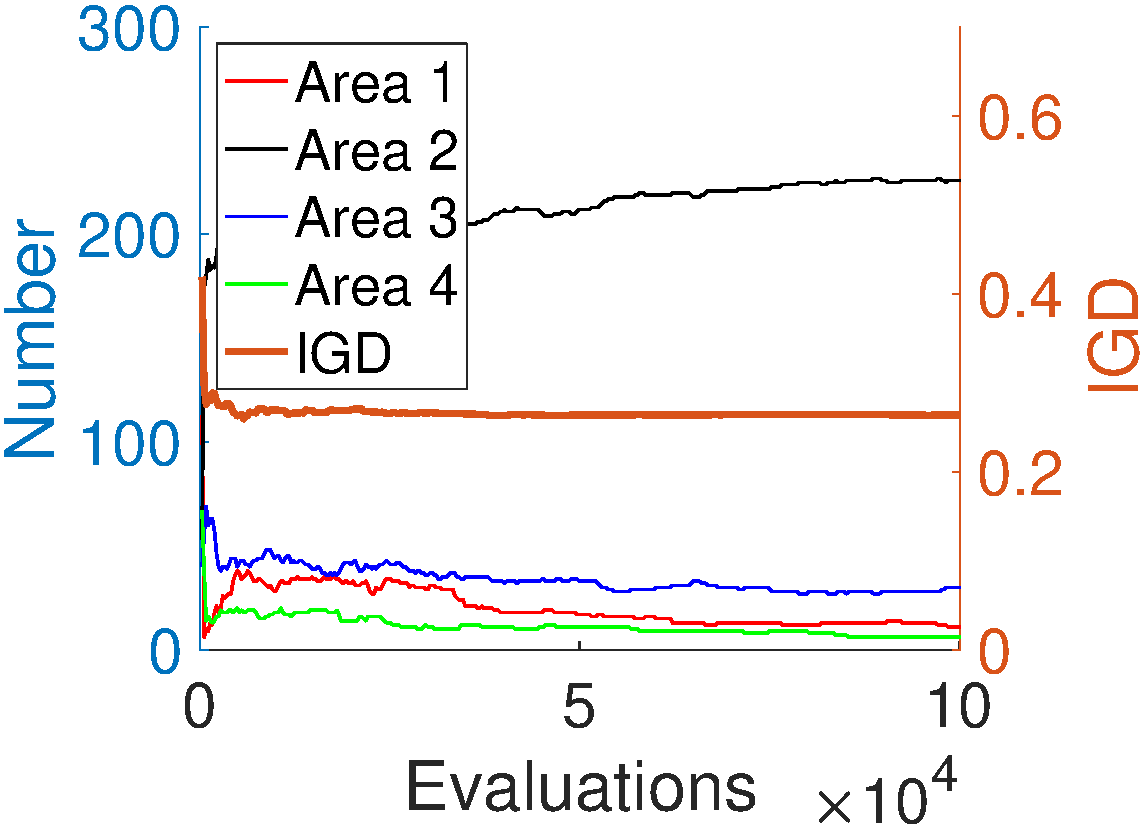
\includegraphics[width=\linewidth]{Section5/dim2/Diversity/MOEAD_TCH}
    \caption{MOEA/D-TCH}
    \label{fig: MOEA/D-TCH Diversity dim=2}
    \end{subfigure}
    
    \begin{subfigure}[b]{.24\textwidth}
    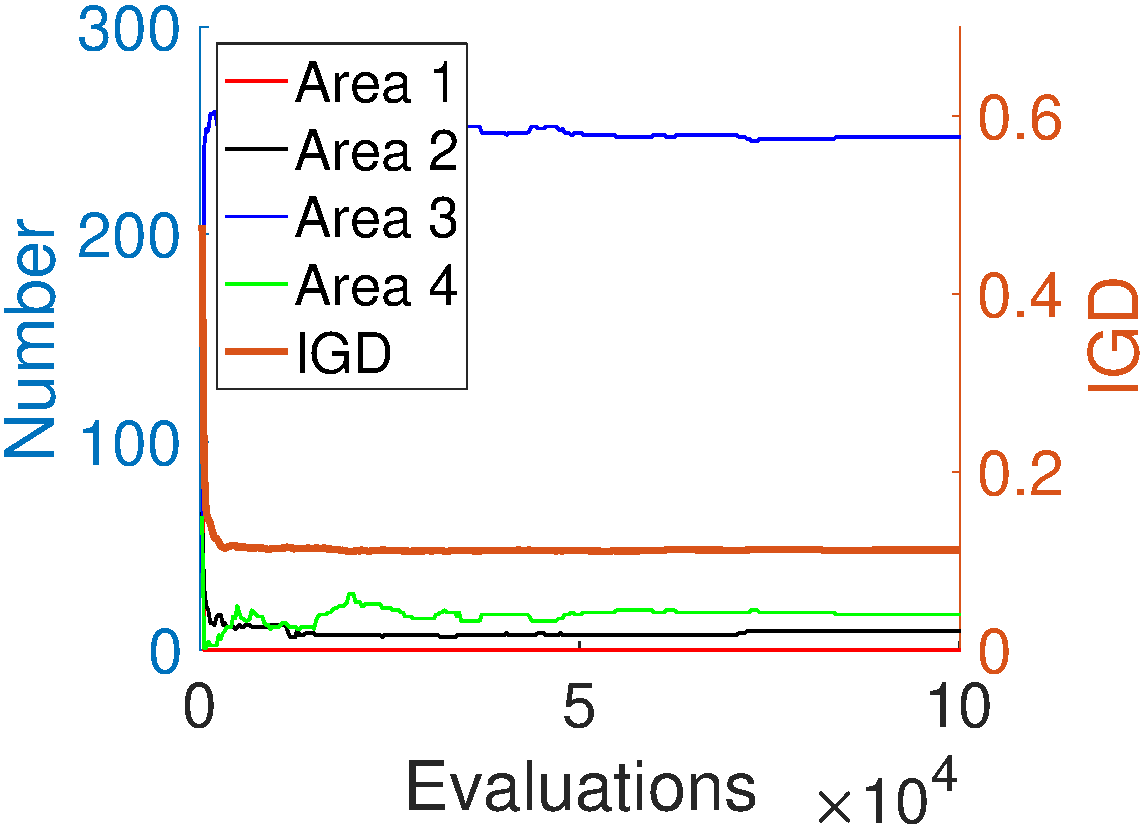
\includegraphics[width=\linewidth]{Section5/dim2/Diversity/MOEAD_PBI}
    \caption{MOEA/D-PBI}
    \label{fig: MOEA/D-PBI Diversity dim=2}
    \end{subfigure}
    \begin{subfigure}[b]{.24\textwidth}
    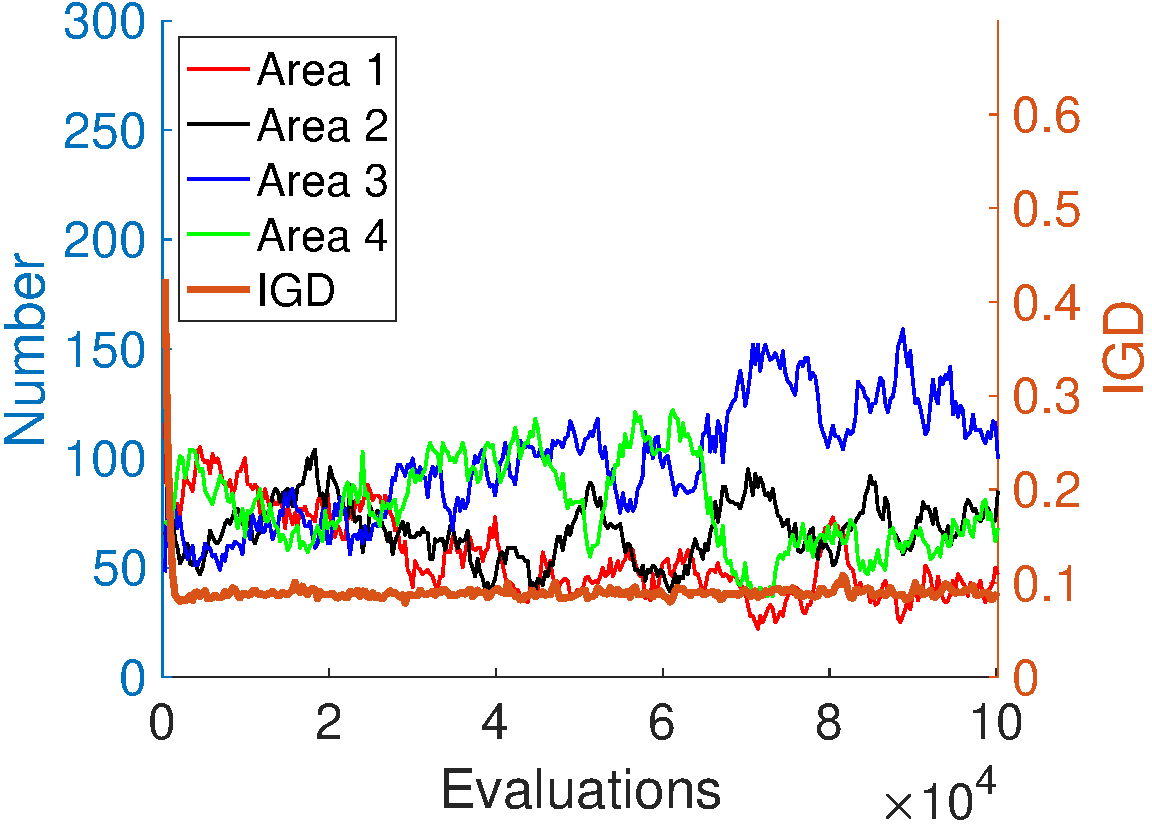
\includegraphics[width=\linewidth]{Section5/dim2/Diversity/IBEA}
    \caption{IBEA}
    \end{subfigure}

    \caption{Solution distribution and IGD value of MOEAs on Multi-Polygon test problem with $D=2$.}
    \label{fig: MOEAs Diversity dim=2}
\end{figure}

\begin{figure}[htbp]
    \centering
    \begin{subfigure}[b]{.24\textwidth}
    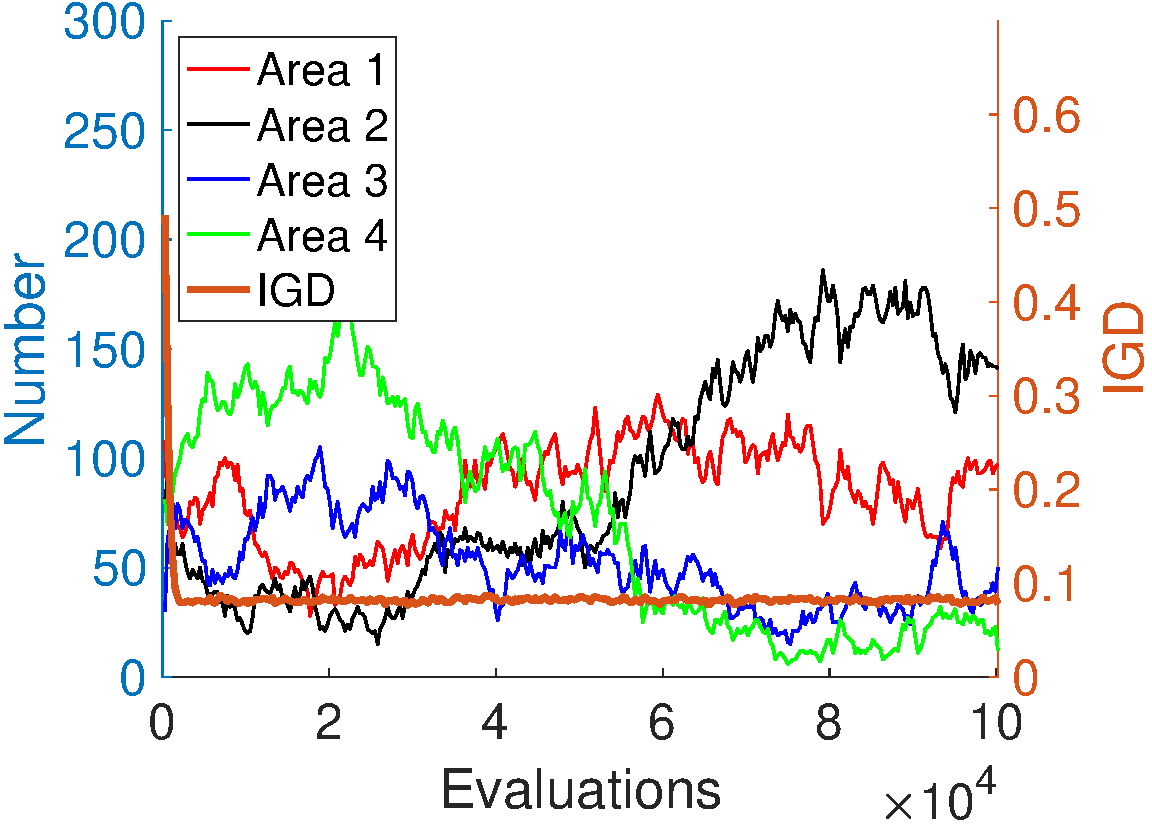
\includegraphics[width=\linewidth]{Section5/dim2/Diversity/DNEA}
    \caption{DNEA}
    \end{subfigure}
    \begin{subfigure}[b]{.24\textwidth}
    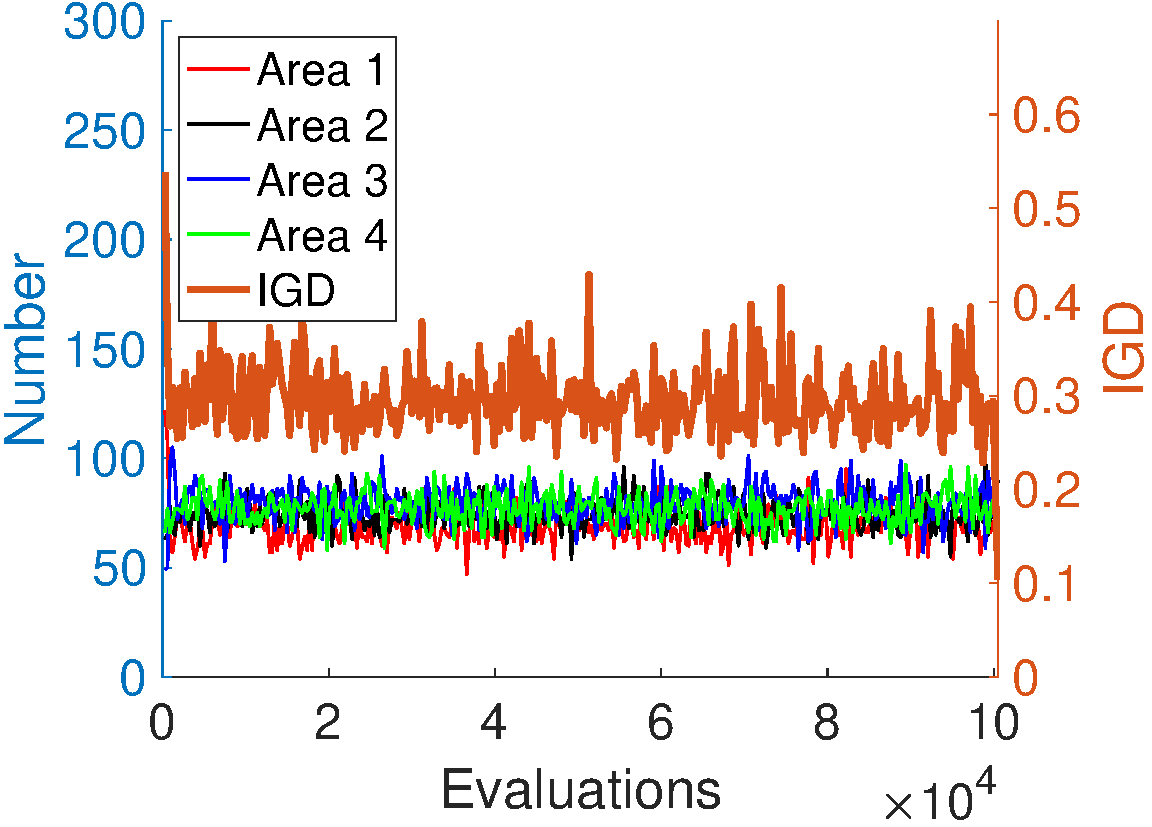
\includegraphics[width=\linewidth]{Section5/dim2/Diversity/MO_Ring_PSO_SCD}
    \caption{MO\_Ring\_PSO\_SCD}
    \end{subfigure}
    
    \begin{subfigure}[b]{.24\textwidth}
    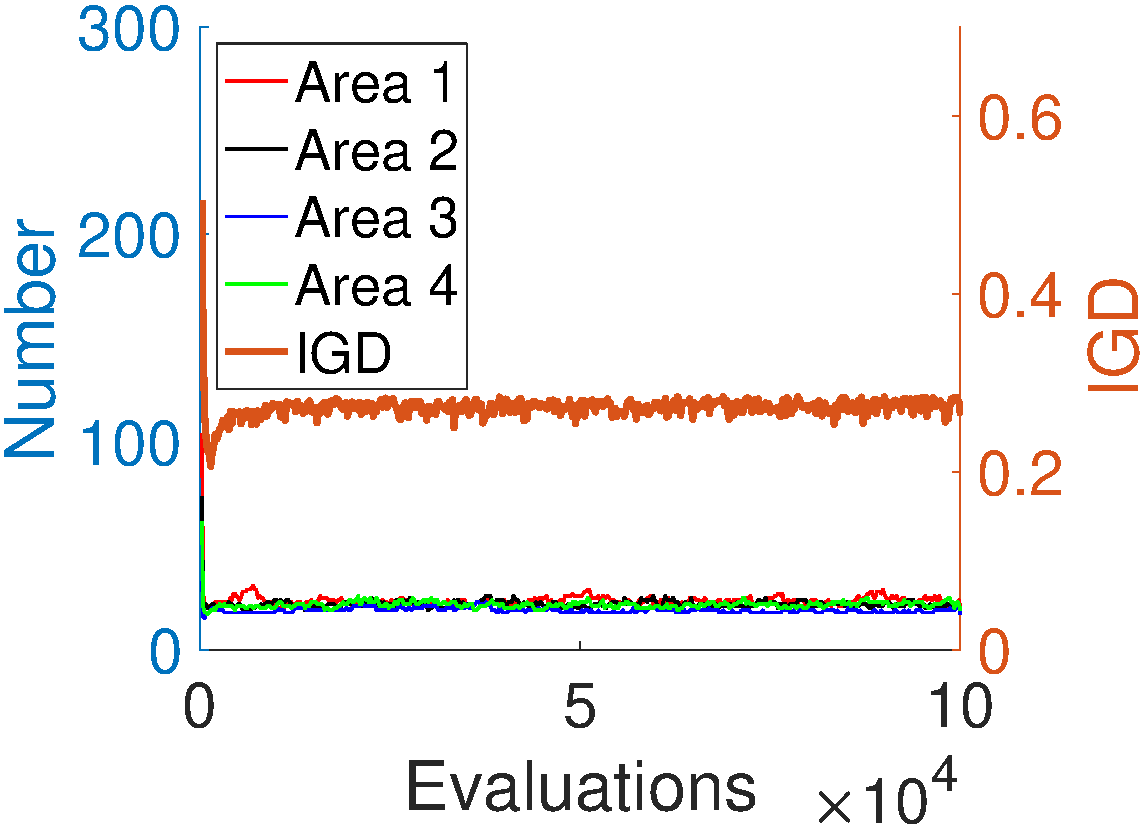
\includegraphics[width=\linewidth]{Section5/dim2/Diversity/MOEADAD}
    \caption{MOEA/D-AD}
    \end{subfigure}
    \begin{subfigure}[b]{.24\textwidth}
    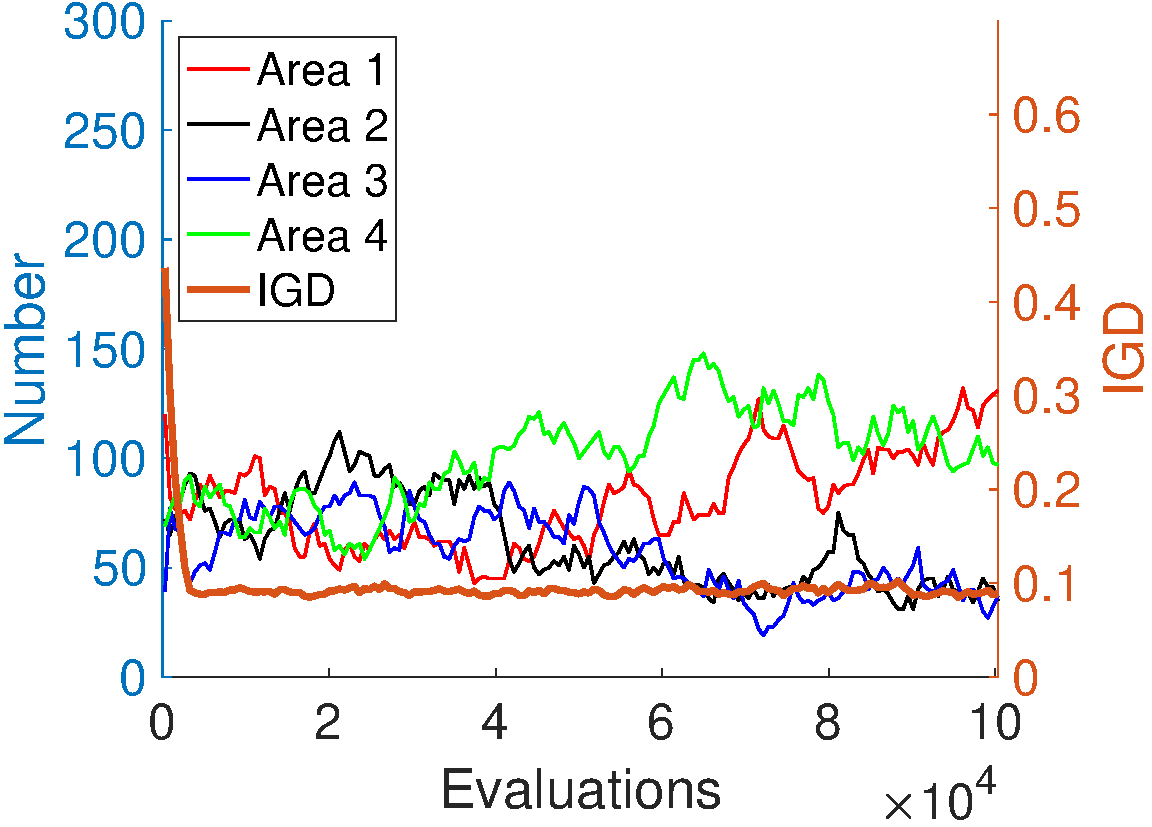
\includegraphics[width=\linewidth]{Section5/dim2/Diversity/OmniOptimizer}
    \caption{Omni-optimizer}
    \end{subfigure}
    \caption{Solution distribution and IGD value of MMEAs on Multi-Polygon test problem with $D=2$.}
    \label{fig: MMEAs Diversity dim=2}
\end{figure}

Figs. \ref{fig: MOEAs Diversity dim=2} and \ref{fig: MMEAs Diversity dim=2} show the solution distribution and IGD value at each epoch for MOEAs and MMEAs respectively. According to figure \ref{fig: MOEAs Diversity dim=2}, for MOEAs which perform good when $D=2$, the number of solutions in each area establishes a "dynamic balance". As shown in Fig. \ref{fig: SBX crossover} (\subref{fig: SBX crossover case 2}), by applying SBX crossover to two solutions in diagonal area will significantly improve the diversity in the decision space. When the number of solutions in diagonal area is very close, a dynamic balance is formed. When the number of solutions in one area is much larger than its diagonal area, dynamic balance cannot be established and only solutions in a single polygon left. Take NSGA-III as an example, in Fig. \ref{fig: MOEAs Diversity dim=2} (\subref{fig: NSGA-III Diversity dim=2}), although the diversity of solution is good at the beginning of the mature stage, most solutions in the final population come from area 3. This is because the third area has much more solutions than others, solutions in other areas quickly disappear. This kind of figures may also help to explain the poor performance of MOEA/D. It can be seen from Figs. \ref{fig: MOEAs Diversity dim=2} (\subref{fig: MOEA/D-TCH Diversity dim=2}) and (\subref{fig: MOEA/D-PBI Diversity dim=2}) that MOEA/D focuses its search in a small area in the decision space at the young stage of evolution. We can conclude that MOEA/D lost its diversity in the decision space because of its environmental selection mechanism.

For MMEAs, the situation that one allele dominates the others never happens when $D=2$. All MMEAs can establish a dynamic balance. Diversity maintenance strategies used in MMEAs are effective in this case.

Following the same manner, we examine the case when $D=4$. The 2-d projection of the final population is shown in Figs. \ref{fig: MOEAs PS dim=4} and \ref{fig: MMEAs PS dim=4}. The simulation results show that it is more difficult to cover all PSs. Most MOEAs only obtain solutions in one or two polygons. For MMEAs, MOEA/D-AD and MO\_Ring\_PSO\_SCD are still able to obtain satisfactory results but the performance of DNEA and Omni-optimizer is worse than our expectations. This shows that the adaptability of fitness sharing and crowding distance approaches is poor. 

%% dim = 4 PS plot 
\begin{figure}[htbp]
    \centering
    \begin{subfigure}[b]{.24\textwidth}
    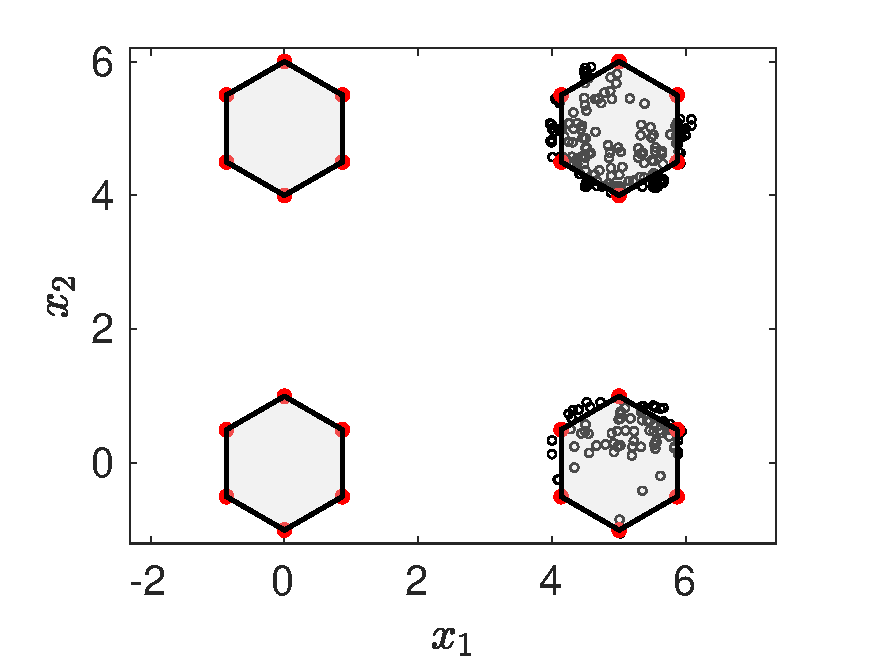
\includegraphics[width=\linewidth]{Section5/dim4/PS/NSGAII}
    \caption{NSGA-II}
    \end{subfigure}
    \begin{subfigure}[b]{.24\textwidth}
    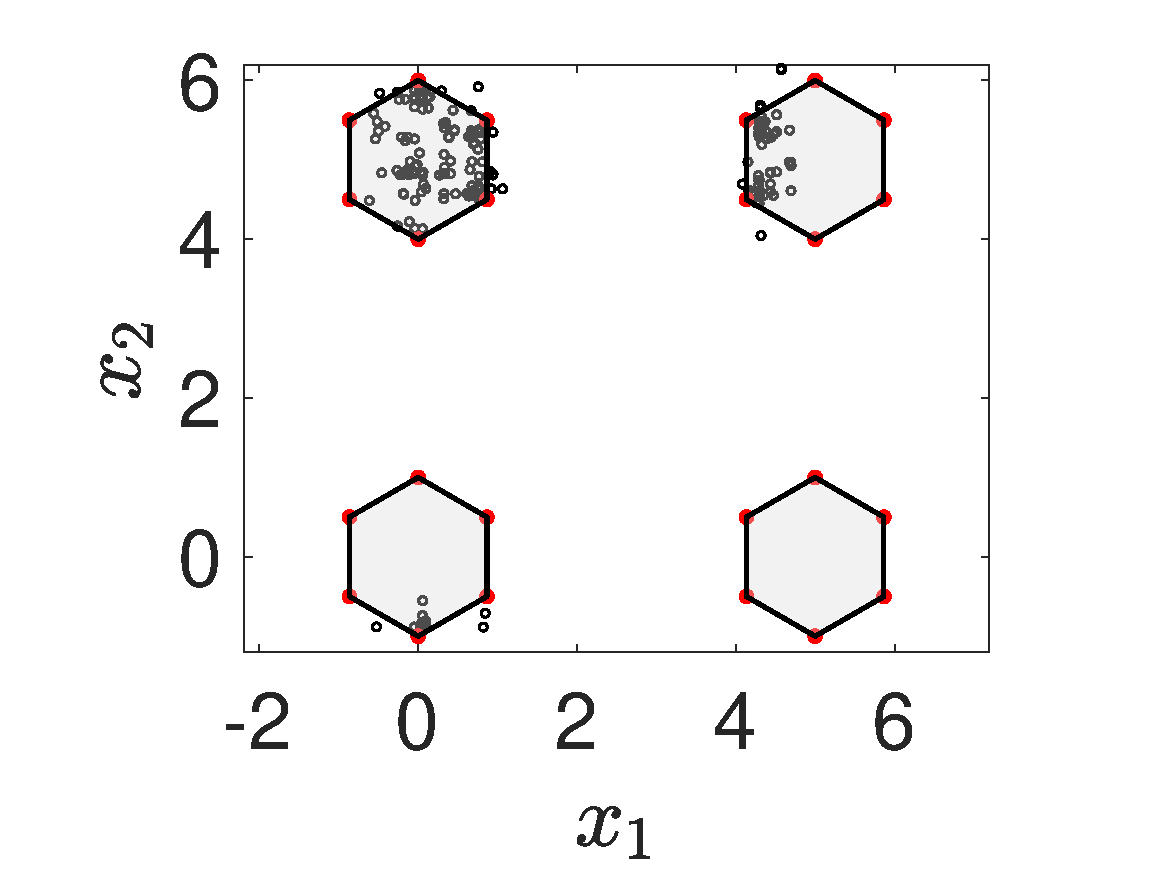
\includegraphics[width=\linewidth]{Section5/dim4/PS/NSGAIII}
    \caption{NSGA-III}
    \end{subfigure}
    
    \begin{subfigure}[b]{.24\textwidth}
    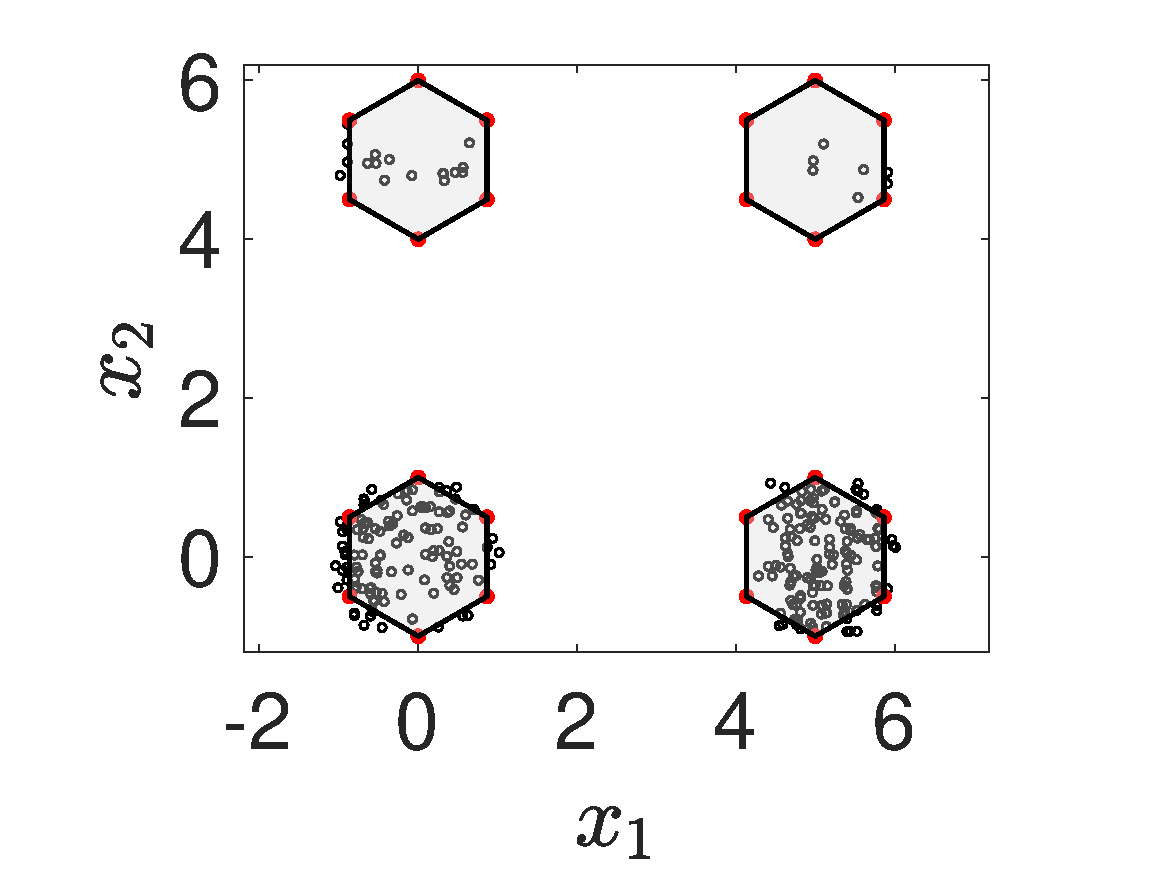
\includegraphics[width=\linewidth]{Section5/dim4/PS/SPEA2}
    \caption{SPEA2}
    \end{subfigure}
    \begin{subfigure}[b]{.24\textwidth}
    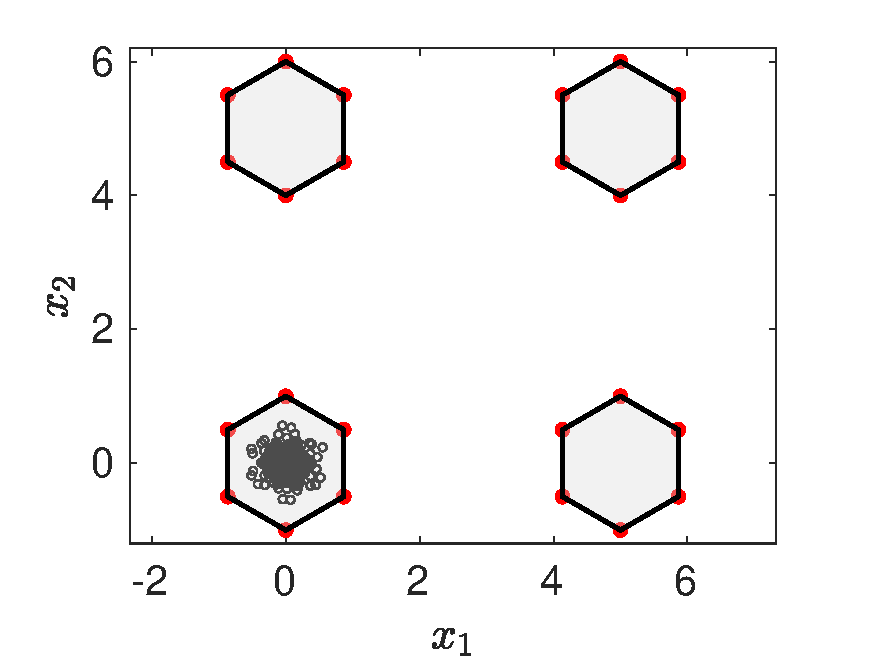
\includegraphics[width=\linewidth]{Section5/dim4/PS/MOEAD_TCH}
    \caption{MOEA/D-TCH}
    \end{subfigure}
    
    \begin{subfigure}[b]{.24\textwidth}
    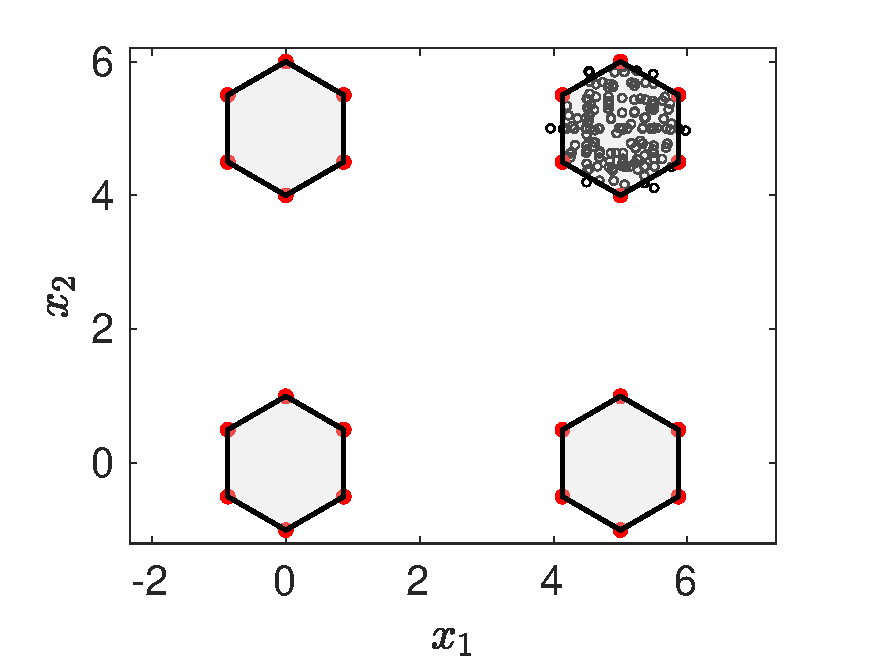
\includegraphics[width=\linewidth]{Section5/dim4/PS/MOEAD_PBI}
    \caption{MOEA/D-PBI}
    \end{subfigure}
    \begin{subfigure}[b]{.24\textwidth}
    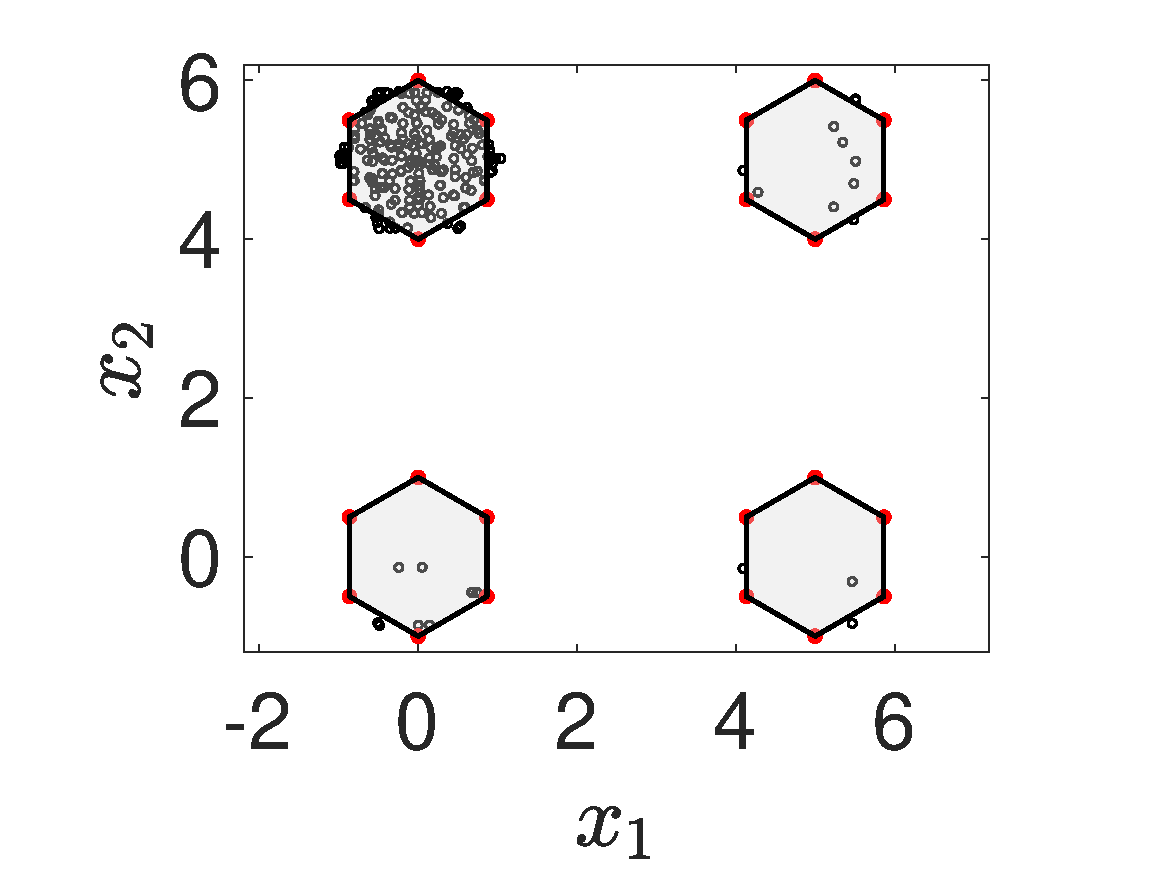
\includegraphics[width=\linewidth]{Section5/dim4/PS/IBEA}
    \caption{IBEA}
    \end{subfigure}

    \caption{Simulation results of MOEAs on Multi-Polygon test problem with $D=4$.}
    \label{fig: MOEAs PS dim=4}
\end{figure}

\begin{figure}[htbp]
    \centering
    \begin{subfigure}[b]{.24\textwidth}
    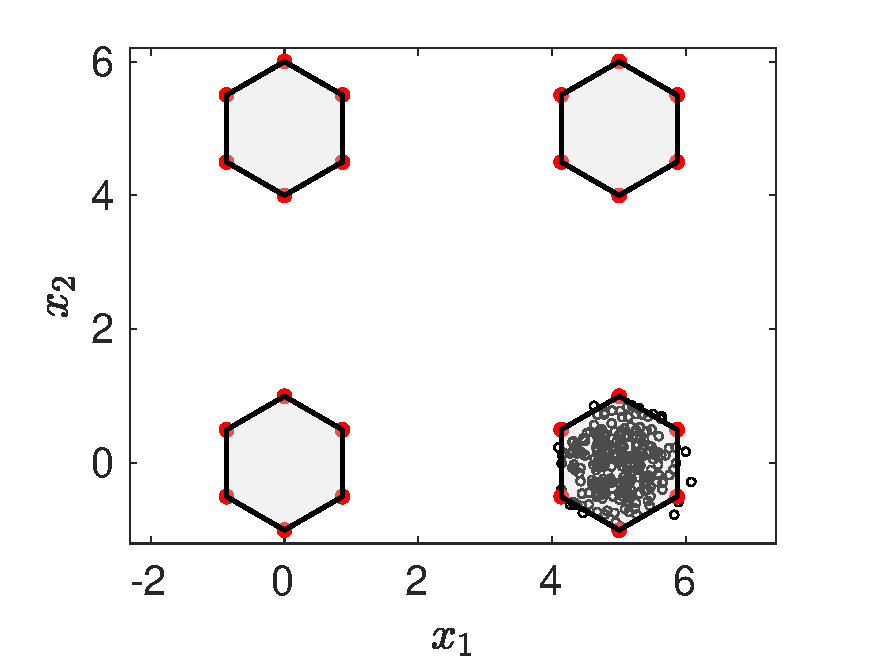
\includegraphics[width=\linewidth]{Section5/dim4/PS/DNEA}
    \caption{DNEA}
    \end{subfigure}
    \begin{subfigure}[b]{.24\textwidth}
    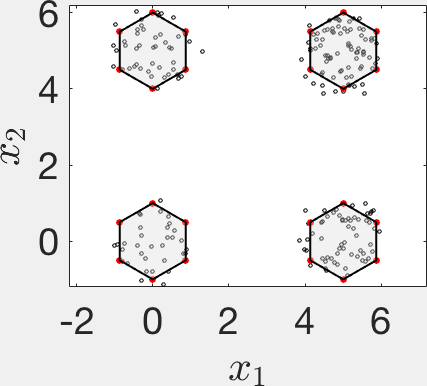
\includegraphics[width=\linewidth]{Section5/dim4/PS/MO_Ring_PSO_SCD}
    \caption{MO\_Ring\_PSO\_SCD}
    \end{subfigure}
    
    \begin{subfigure}[b]{.24\textwidth}
    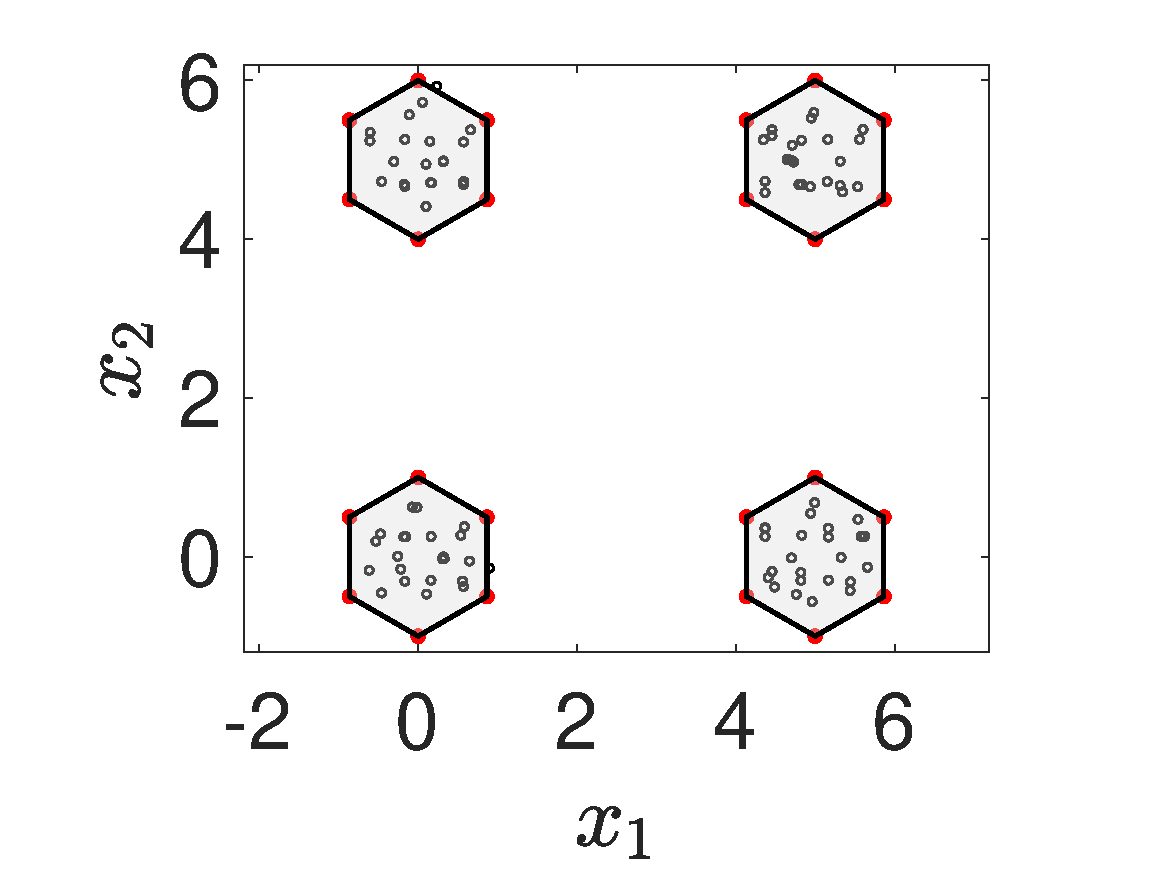
\includegraphics[width=\linewidth]{Section5/dim4/PS/MOEADAD}
    \caption{MOEA/D-AD}
    \end{subfigure}
    \begin{subfigure}[b]{.24\textwidth}
    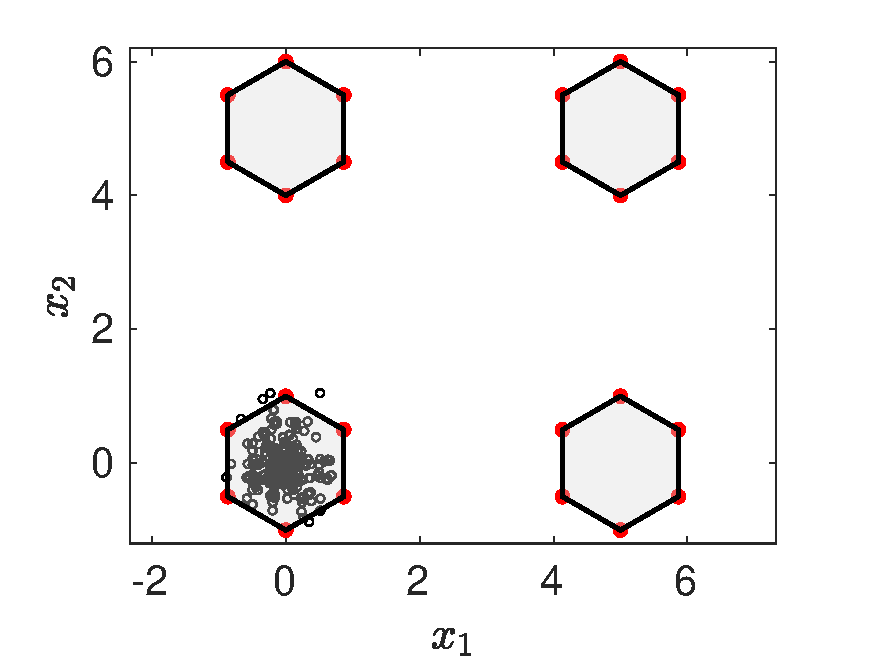
\includegraphics[width=\linewidth]{Section5/dim4/PS/OmniOptimizer}
    \caption{Omni-optimizer}
    \end{subfigure}
    \caption{Simulation results of MMEAs on Multi-Polygon test problem with $D=4$.}
    \label{fig: MMEAs PS dim=4}
\end{figure}

We also examine the distribution of solutions in the decision space during the evolution. According to Figs. \ref{fig: MOEAs Diversity dim=4} and \ref{fig: MMEAs Diversity dim=4}, we can see that when $D=4$, it is harder to establish dynamic balance than $D=2$ and the magnitude of the change of the number of solutions in each area is small. According to Fig. \ref{fig: MMEAs Diversity dim=4}, the diversity of the population in the decision space of DNEA and Omni-optimizer quickly disappears. These two MMEAs are unable to maintain the diversity of the population in the decision space when $D=4$. 

%% dim = 4 Diversity Plot
\begin{figure}[htbp]
    \centering
    \begin{subfigure}[b]{.24\textwidth}
    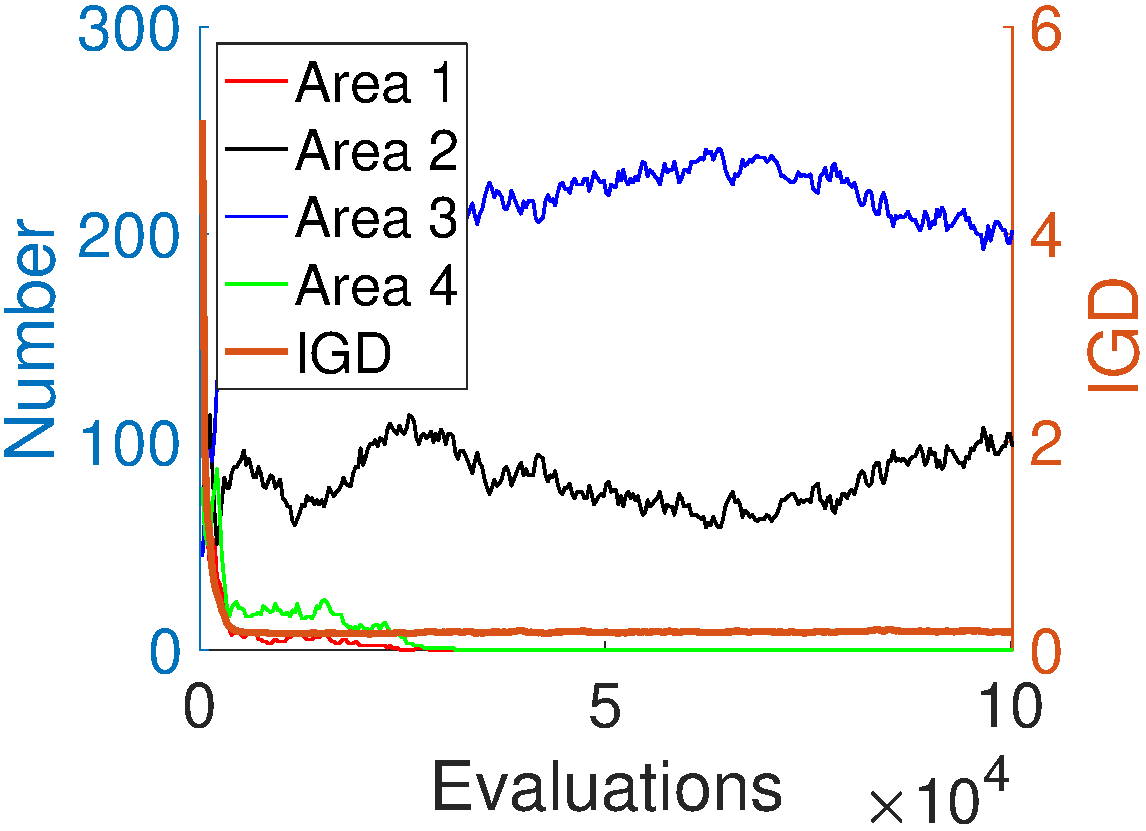
\includegraphics[width=\linewidth]{Section5/dim4/Diversity/NSGAII}
    \caption{NSGA-II}
    \end{subfigure}
    \begin{subfigure}[b]{.24\textwidth}
    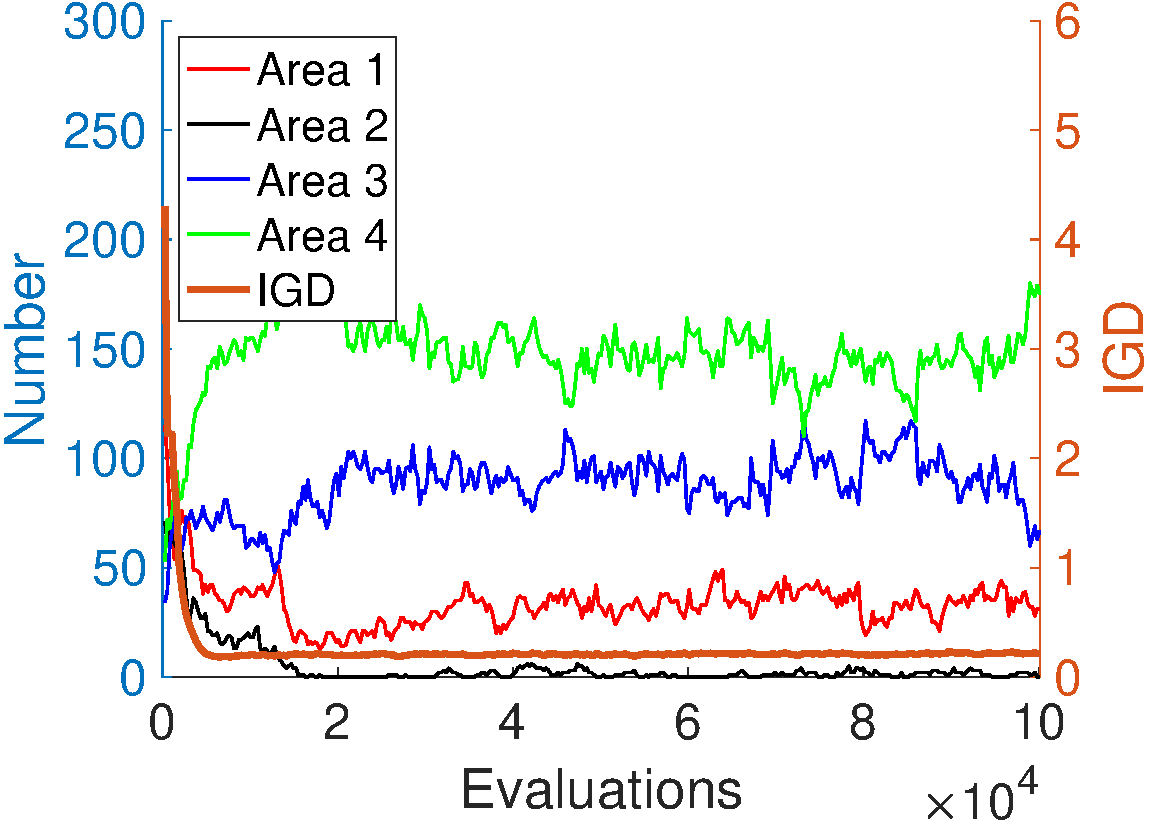
\includegraphics[width=\linewidth]{Section5/dim4/Diversity/NSGAIII}
    \caption{NSGA-III}
    \end{subfigure}
    
    \begin{subfigure}[b]{.24\textwidth}
    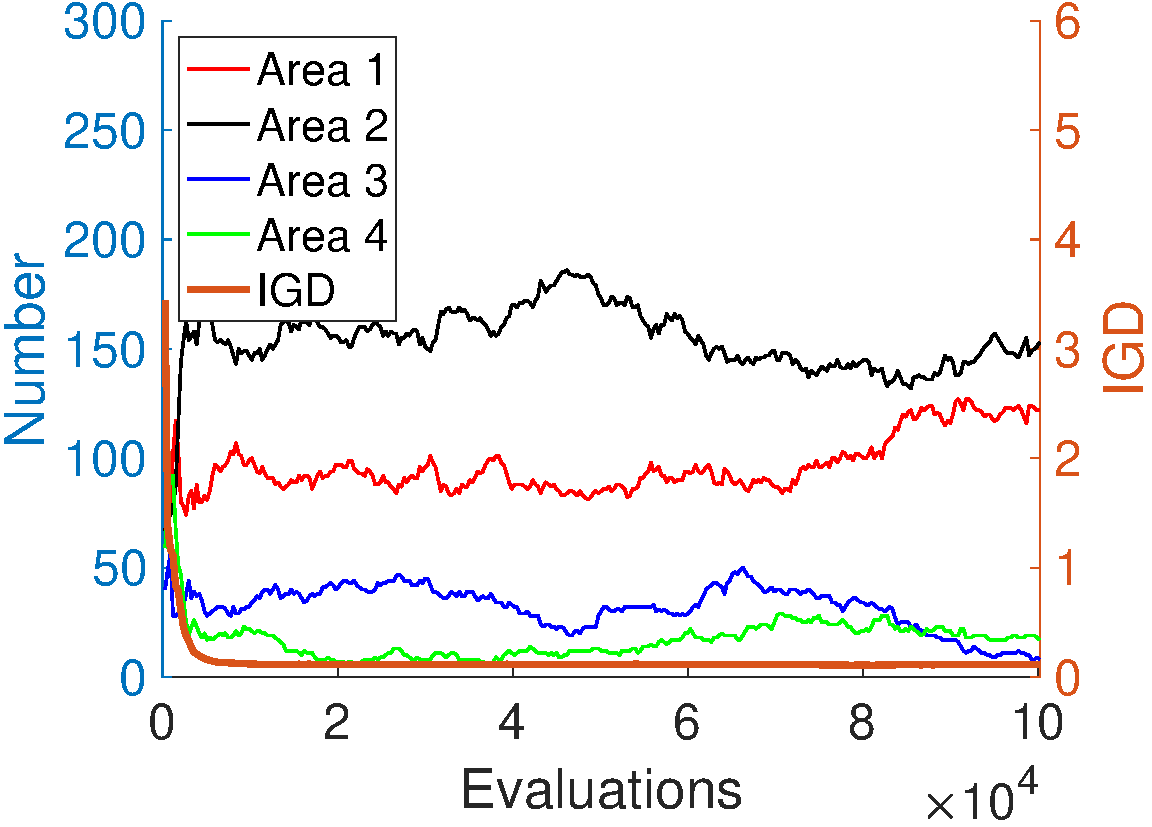
\includegraphics[width=\linewidth]{Section5/dim4/Diversity/SPEA2}
    \caption{SPEA2}
    \end{subfigure}
    \begin{subfigure}[b]{.24\textwidth}
    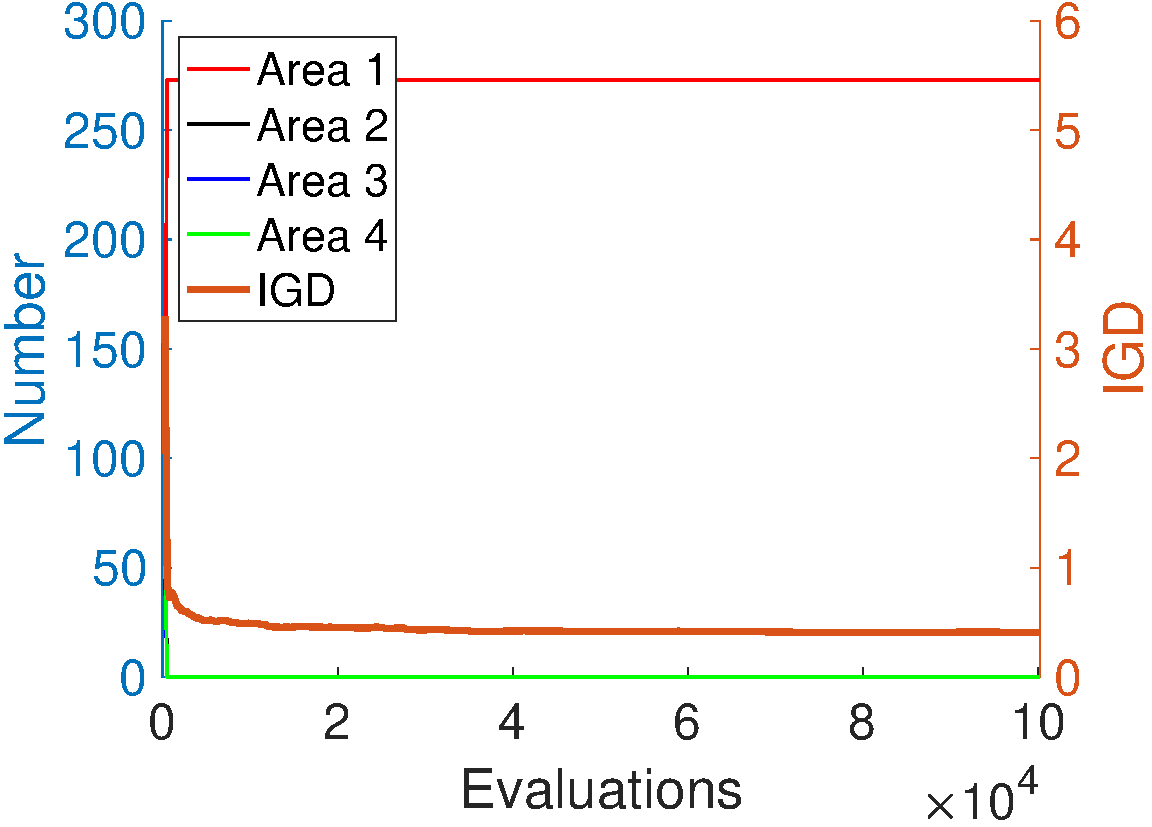
\includegraphics[width=\linewidth]{Section5/dim4/Diversity/MOEAD_TCH}
    \caption{MOEA/D-TCH}
    
    \end{subfigure}
    \begin{subfigure}[b]{.24\textwidth}
    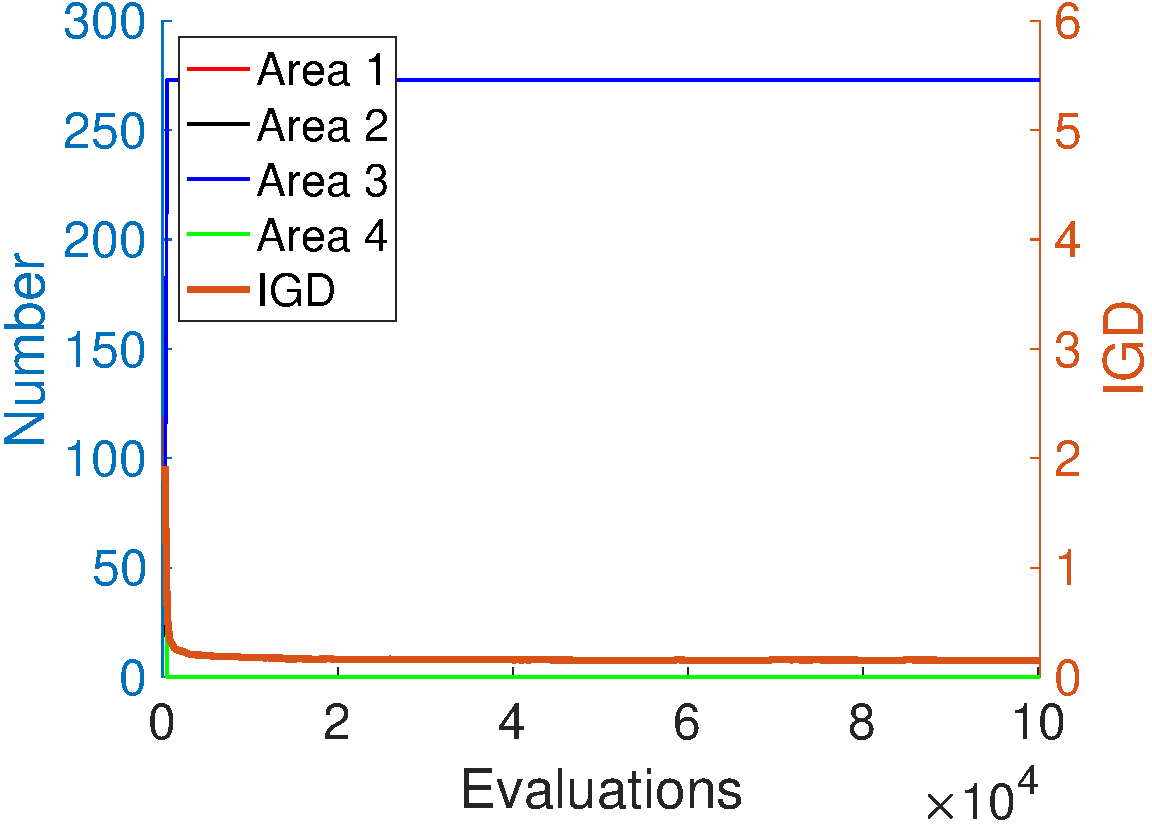
\includegraphics[width=\linewidth]{Section5/dim4/Diversity/MOEAD_PBI}
    \caption{MOEA/D-PBI}
    \end{subfigure}
    \begin{subfigure}[b]{.24\textwidth}
    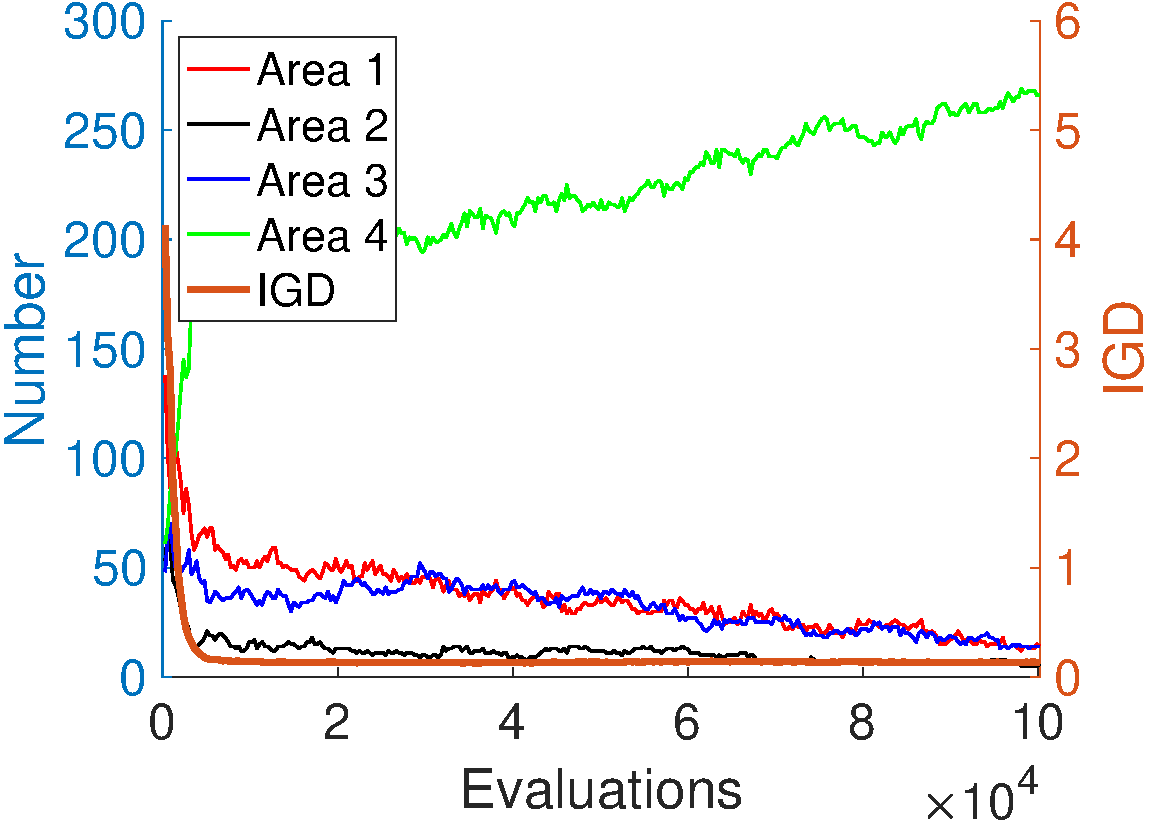
\includegraphics[width=\linewidth]{Section5/dim4/Diversity/IBEA}
    \caption{IBEA}
    \end{subfigure}

    \caption{Solution distribution and IGD value of MOEAs on Multi-Polygon test problem with $D=4$.}
    \label{fig: MOEAs Diversity dim=4}
\end{figure}

\begin{figure}[htbp]
    \centering
    \begin{subfigure}[b]{.24\textwidth}
    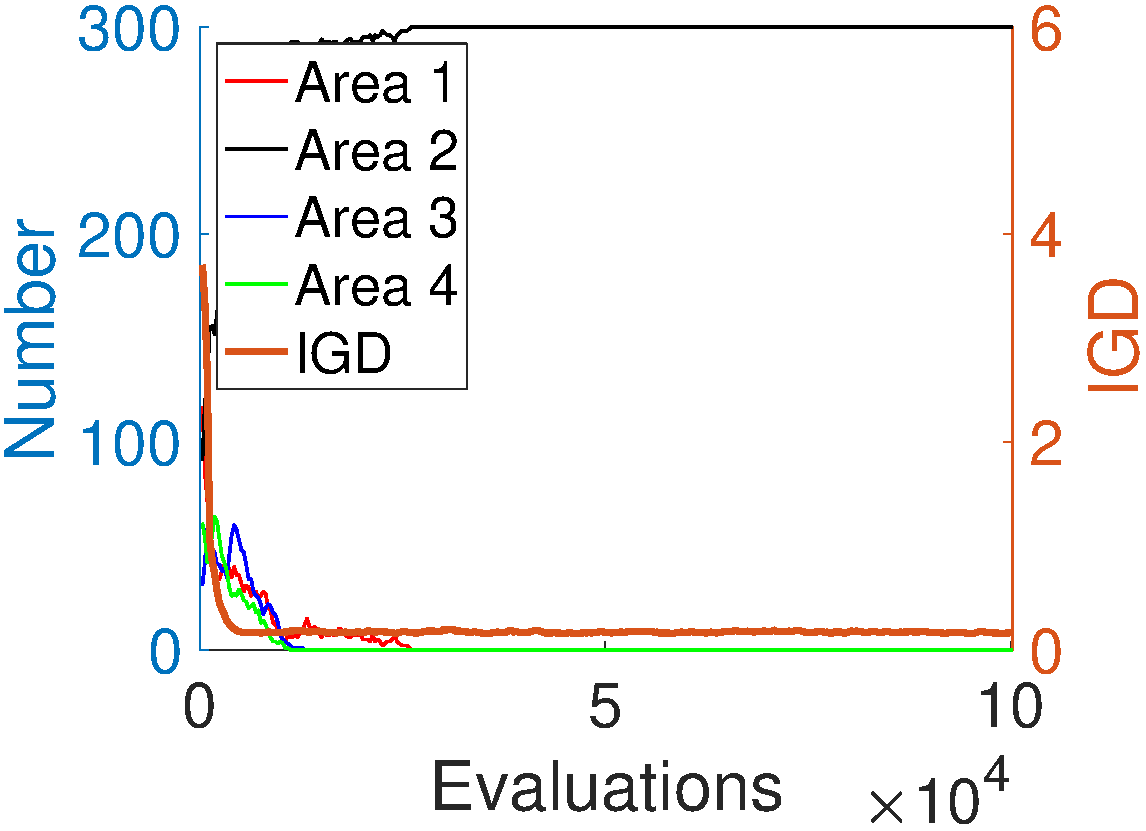
\includegraphics[width=\linewidth]{Section5/dim4/Diversity/DNEA}
    \caption{DNEA}
    \end{subfigure}
    \begin{subfigure}[b]{.24\textwidth}
    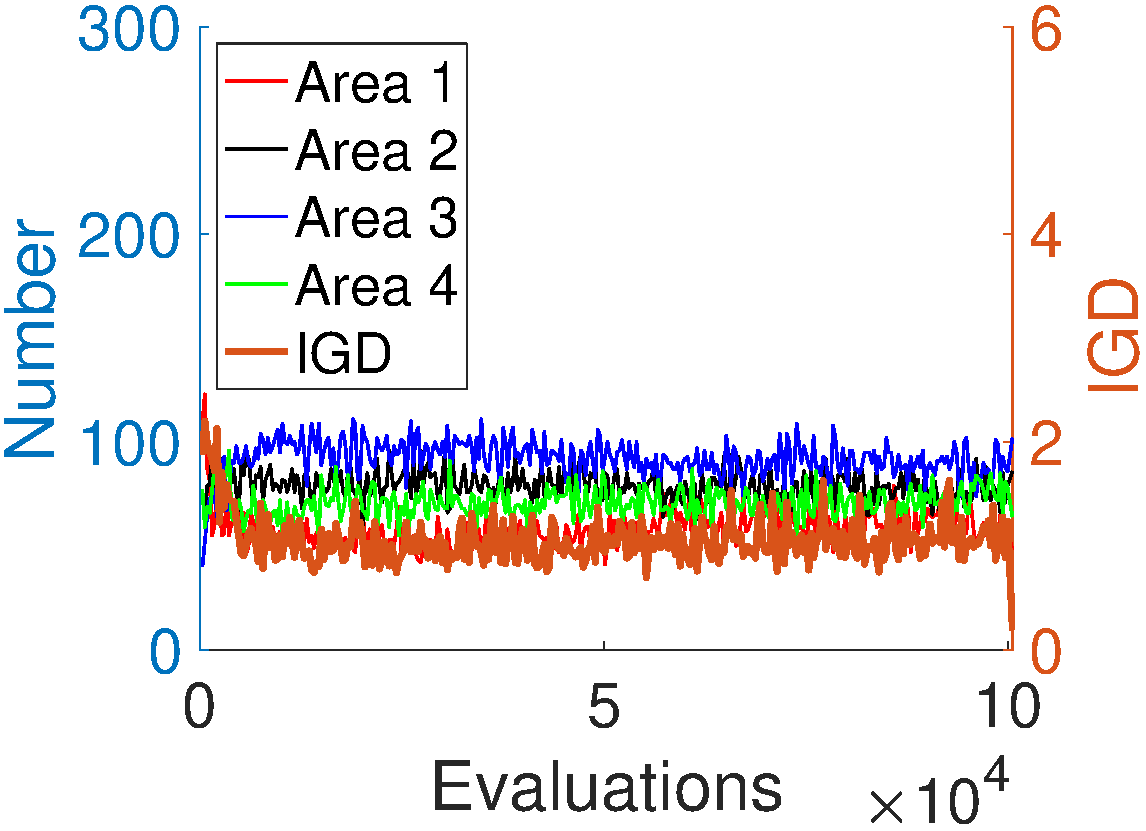
\includegraphics[width=\linewidth]{Section5/dim4/Diversity/MO_Ring_PSO_SCD}
    \caption{MO\_Ring\_PSO\_SCD}
    \end{subfigure}
    
    \begin{subfigure}[b]{.24\textwidth}
    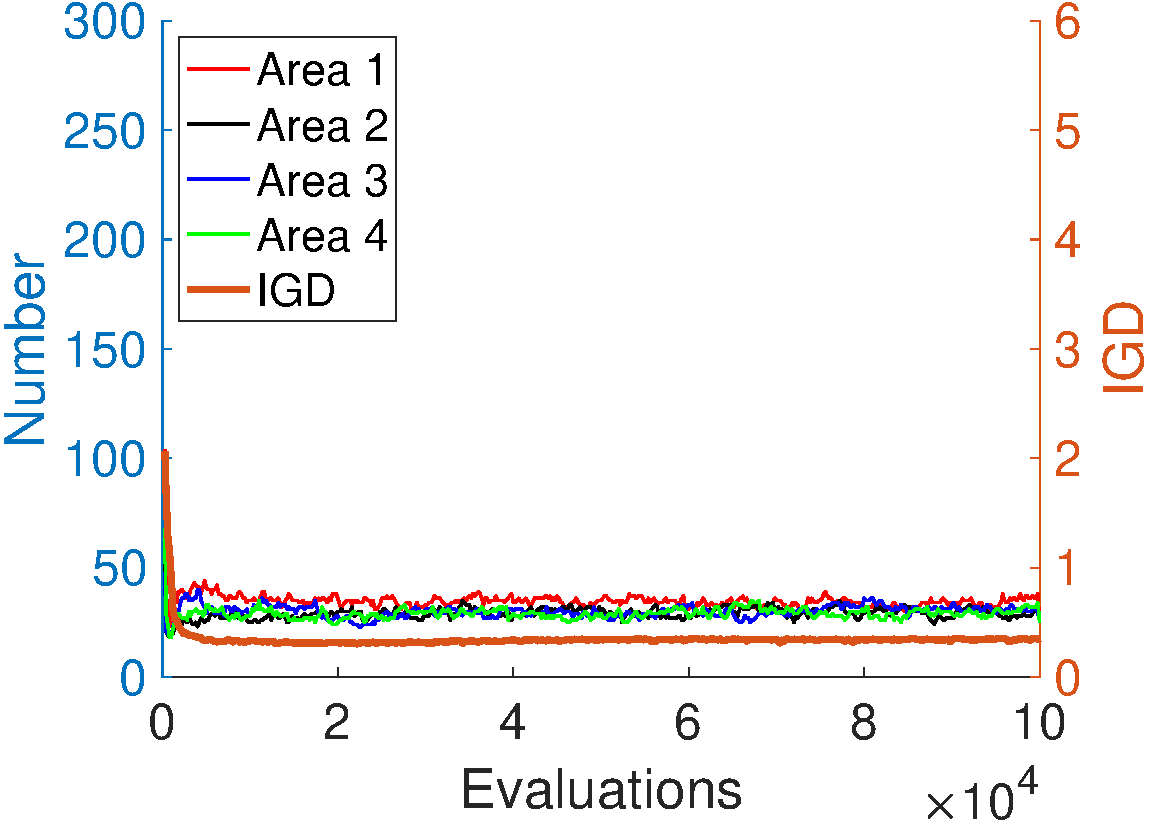
\includegraphics[width=\linewidth]{Section5/dim4/Diversity/MOEADAD}
    \caption{MOEA/D-AD}
    \end{subfigure}
    \begin{subfigure}[b]{.24\textwidth}
    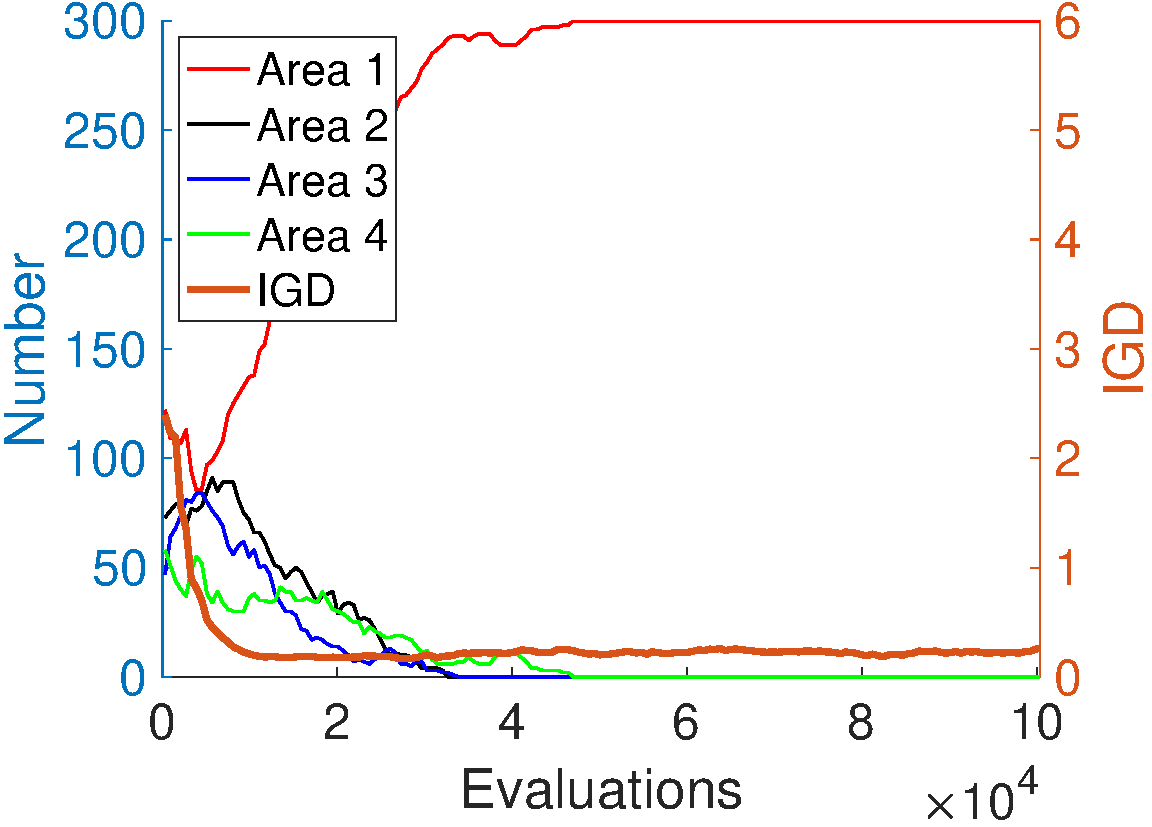
\includegraphics[width=\linewidth]{Section5/dim4/Diversity/OmniOptimizer}
    \caption{Omni-optimizer}
    \end{subfigure}
    \caption{Solution distribution and IGD value of MMEAs on Multi-Polygon test problem with $D=4$.}
    \label{fig: MMEAs Diversity dim=4}
\end{figure}

Due to the page limitation, the simulation results of MOEAs and MMEAs on Multi-Polygons test problem with higher dimensional decision space are not shown here. Instead, we show IGD and IGDX\cite{Liang2016} values of each algorithm when $D=2, 4, 6, 8, 10, 100$. These two indicators measure the quality of the solution set in the objective and decision space respectively. Notice that the best values in each table are highlighted in yellow. From Table \ref{table: IGDX sumup}, it is obvious that MO\_Ring\_PSO\_SCD and MOEA/D-AD have much smaller IGDX values than others which means that the quality of the obtained solutions have better coverage in the decision space. These indicator values are consistent with our visualization results.

\begin{table}[htbp]
\centering
\caption{IGDX values}
\begin{tabular}{@{}ccccccc@{}}
\toprule
Algorithms      & D=2                          & D=4                          & D=6                          & D=8                          & D=10                         & D=100                         \\ \midrule
NSGA-II         & 0.14                         & 2.71                         & 4.81                         & 6.67                         & 8.09                         & 28.44                         \\
NSGA-III        & 1.53                         & 3.4                          & 5.2                          & 6.87                         & 8.15                         & 29.56                         \\
SPEA2           & \cellcolor[HTML]{F8FF00}0.11 & 1.84                         & 4.74                         & 6.87                         & 7.85                         & \cellcolor[HTML]{F8FF00}28.45 \\
MOEA/D-TCH      & 1.17                         & 5.53                         & 6.91                         & 8.13                         & 9.22                          & 31.06                         \\
MOEA/D-PBI      & 1.96                         & 4.96                         & 6.29                         & 7.32                         & 8.26                         & 29.73                         \\
IBEA            & 0.13                         & 1.8                          & 5.03                         & 6.91                         & 7.82                         & 29.52                         \\
DNEA            & 0.12                         & 5.13                         & 6.49                         & 7.69                         & 8.73                         & 30.74                         \\
MO\_Ring\_PSO\_SCD & \cellcolor[HTML]{F8FF00}0.11 & 0.33                         & 0.68                         & 1.13                         & 1.9                          & 44.08                         \\
MOEA/D-AD       & 0.19                         & \cellcolor[HTML]{F8FF00}0.28 & \cellcolor[HTML]{F8FF00}0.41 & \cellcolor[HTML]{F8FF00}0.57 & \cellcolor[HTML]{F8FF00}0.82 & 32.96                         \\
Omni-optimizer  & 0.16                         & 5.08                         & 6.47                         & 7.83                         & 9.02                         & 30.62                         \\ \bottomrule
\end{tabular}
\label{table: IGDX sumup}
\end{table}
 However, from the perspective of objective space, the situation is different. As shown in Table \ref{table: IGD sumup}, the IGD values of MMEAs are usually larger than MOEAs especially when $D$ is large. IBEA and SPEA2 outperform others in terms of the quality of solutions in the objective space. This observation has been reported in \cite{MO-Ring-PSO-SCD} and \cite{Shir:2009dz}. The reasons are mainly from two aspects. Firstly, suppose an MMOP has $K$ equivalent Pareto sets and an MMEA contains $N$ individuals. Ideally, this MMEA only uses $1/K$ of $N$ individuals to locate each Pareto set,  which means that this MMEA is equivalent to an MOEA with population size = $N/K$. Smaller population size usually means weaker search power. Secondly, the value of IGD indicator is also related to the number of individuals in PF approximation. For example, suppose that solutions sets $S_1$ and $S_2$ are uniformly spread along the PF. If $S_1$ contains more individuals than $S_2$, then usually $IGD(S_1) < IGD(S_2)$. In Table \ref{table: Perpendicular Distance}, we show the average perpendicular distances of solutions to the target plane for each algorithm. It is clear that solutions obtained by the two best MMEAs: MOEA/D-AD and MO\_Ring\_PSO\_SCD are further to the target plane than most other MOEAs.

\begin{table}[htbp]
\centering
\caption{IGD values}
\begin{tabular}{@{}ccccccc@{}}
\toprule
Algorithms      & D=2                          & D=4                          & D=6                          & D=8                          & D=10                        & D=100                        \\ \midrule
NSGA-II         & 0.1                          & 0.17                         & 0.25                         & 0.33                         & 0.41                        & 3.01                         \\
NSGA-III        & 0.14                         & 0.21                         & 0.28                         & 0.33                         & 0.39                        & 3.95                         \\
SPEA2           & \cellcolor[HTML]{F8FF00}0.07 & \cellcolor[HTML]{F8FF00}0.12 & 0.16                         & 0.2                          & 0.24                        & \cellcolor[HTML]{F8FF00}2.73 \\
MOEA/D-TCH      & 0.26                         & 0.41                         & 0.64                         & 0.93                         & 1.2                         & 6.76                         \\
MOEA/D-PBI      & 0.11                         & 0.16                         & 0.2                          & 0.25                         & 0.3                         & 4.22                          \\
IBEA            & 0.09                         & 0.13                         & \cellcolor[HTML]{F8FF00}0.15 & \cellcolor[HTML]{F8FF00}0.17 & \cellcolor[HTML]{F8FF00}0.2 & 3.9                          \\
DNEA            & 0.08                         & 0.17                         & 0.31                         & 0.5                          & 0.67                        & 5.91                         \\
MO\_Ring\_PSO\_SCD & 0.1                          & 0.19                         & 0.4                          & 0.72                         & 1.12                        & 57.46                        \\
MOEA/D-AD       & 0.27                         & 0.36                         & 0.47                         & 0.58                         & 0.72                        & 12.97                        \\
Omni-optimizer  & 0.09                         & 0.22                          & 0.45                         & 0.7                          & 0.95                        & 5.54                         \\ \bottomrule
\end{tabular}
\label{table: IGD sumup}
\end{table}

\begin{table}[htbp]
\centering
\caption{Average perpendicular distances}
\begin{tabular}{@{}ccccccc@{}}
\toprule
Algorithms         & D=2 & D=4                           & D=6                           & D=8                           & D=10                          & D=100                         \\ \midrule
NSGA-II            & 0  & 0.18                         & 0.31                         & 0.41                         & 0.57                         & 3.85                         \\
NSGA-III           & 0  & 0.18                         & 0.31                         & 0.39                         & 0.48                         & 2.77                         \\
SPEA2              & 0  & 0.18                         & 0.3                          & 0.41                         & 0.49                         & 2.98                         \\
MOEA/D-TCH         & 0  & \cellcolor[HTML]{F8FF00}0.01 & \cellcolor[HTML]{F8FF00}0.05 & \cellcolor[HTML]{F8FF00}0.05 & \cellcolor[HTML]{F8FF00}0.07 & \cellcolor[HTML]{F8FF00}0.31 \\
MOEA/D-PBI         & 0  & 0.08                         & 0.16                         & 0.25                         & 0.3                          & 1.53                         \\
IBEA               & 0  & 0.03                         & 0.06                         & 0.12                         & 0.18                         & 1.61                         \\
DNEA               & 0  & 0.23                         & 0.36                         & 0.43                         & 0.5                          & 1.37                         \\
MO\_Ring\_PSO\_SCD & 0  & 0.28                         & 0.66                         & 1.05                         & 1.43                         & 32.01                        \\
MOEA/D-AD          & 0  & 0.09                         & 0.18                         & 0.31                         & 0.48                         & 10.26                        \\
Omni-optimizer     & 0  & 0.22                      & 0.31                         & 0.4                          & 0.41                         & 2.68                         \\ \bottomrule
\end{tabular}
\label{table: Perpendicular Distance}
\end{table}
\section{Concluding Remarks}
\label{Conclusion}
This paper mainly made two contributions. Firstly, we addressed the difficulties of solving MMOPs in detail. We pointed out that the selection, mutation and crossover operations in classical MOEAs will cause problems when handling MMOPs. Furthermore, genetic drift concept was introduced to explain the the phenomenon of the diversity loss in the decision space during evolution. Our analysis may help to develop new algorithms for solving MMOPs.

Secondly, a series of computational experiments were conducted to examine the performance of MOEAs and MMEAs on Multi-Polygon test problem with different dimensional decision spaces. The experimental results showed that the adaptability of DNEA and Omni-optimizer is poor. Another two MMEAs MO\_Ring\_PSO\_SCD and MOEA/D-AD can effectively preserve the diversity in the decision space compared with DNEA, Omni-optimizer and other MOEAs. We also showed that maintaining the diversity in the decision space will cause deterioration of the search power by comparing the IGD values and average perpendicular distance of MMEAs with MOEAs. 

In future research, more experiments are needed to clearly show the effect of diversity maintenance mechanisms in the decision space on the search ability of an MMEA.

\section*{Acknowledgment}
This work was supported by National Natural Science Foundation of China (Grant No. 61876075), the Program for Guangdong Introducing Innovative and Entrepreneurial Teams (Grant No. 2017ZT07X386), Shenzhen Peacock Plan (Grant No. KQTD2016112514355531), the Science and Technology Innovation Committee Foundation of Shenzhen (Grant No. ZDSYS201703031748284), the Program for University Key Laboratory of Guangdong Province (Grant No. 2017KSYS008).
\bibliographystyle{ieeetr}
\bibliography{References.bib}

\end{document}
